\documentclass[a4paper,11pt,oneside,titlepage]{article}
\usepackage{a4wide}
\usepackage[utf8]{inputenc}
\usepackage[T1]{fontenc}
\usepackage[french]{babel}
\usepackage{tikz-cd}
\usepackage{quiver}
\usetikzlibrary{decorations.pathmorphing}
\usetikzlibrary{babel}
\usepackage{xcolor}
\usepackage{csquotes}
\usepackage[framemethod=TikZ]{mdframed}
\usepackage{graphicx}
\usepackage{amssymb}
\usepackage{amsmath}
\usepackage{amsthm}
\usepackage[margin=2.5cm]{geometry}
\pagestyle{headings}
\usepackage{yfonts}
\usepackage[colorlinks=true,allcolors=black]{hyperref}
\usepackage{subcaption}
\usepackage[backend=biber,style=numeric]{biblatex}
\DeclareBibliographyCategory{utilises}
\DeclareBibliographyCategory{plusloin}
\addbibresource{refs.bib}
\renewcommand{\tilde}[1]{\widetilde{#1}}
\renewcommand{\vec}[1]{\overrightarrow{#1}}
\renewcommand{\bar}[1]{\overline{#1}}
\renewcommand{\underbar}[1]{\underline{#1}}
\usepackage[most]{tcolorbox}



\newtcolorbox{equivbox}[1]{
  colback=gray!5,
  colframe=black,
  fonttitle=\bfseries,
  title=#1,
  boxrule=0.8pt,
  arc=2pt
}
\renewcommand{\familydefault}{qhv}

\newcommand{\rightan}[3]{TR_{#1}}
\newcommand{\rightane}[3]{TR_{#1}^e}
\newcommand{\lefttan}[3]{TL_{#1}}
\newcommand{\lefttane}[3]{TL_{#1}^e}
\newcommand{\conttan}[3]{TK_{#1}}
\newcommand{\conttane}[3]{TK_{#1}^{e}}
\newcommand{\fibltan}[3]{TC_{#1}}
\newcommand{\gentan}[3]{TG_{#1}}
\newcommand{\todo}[1]{\textcolor{red}{TO DO [}#1\textcolor{red}{]}}


\newcommand{\todomaybe}[1]{\textcolor{orange}{TO DO ? [}#1\textcolor{orange}{]}}

\newcommand{\R}[0]{\mathbb{R}}

\newcommand{\nul}[0]{\operatorname{nul}}

\newcommand{\im}[0]{\operatorname{im}}
\newcommand{\coker}[0]{\operatorname{coker}}
\newcommand{\coim}[0]{\operatorname{coim}}
\newcommand{\id}[0]{\operatorname{Id}}
\newcommand{\de}[0]{\operatorname{def}}


\tcbuselibrary{theorems,breakable}


\newtcbtheorem[number within=section]{theobox}{Théorème}
{colback=white,
 colframe=color-prop,
 fonttitle=\bfseries,
 enhanced,
 attach boxed title to top left={xshift=2mm,yshift=-2mm},
 boxed title style={colback=color-prop},
 separator sign none,
 description delimiters={(}{)},
}{th}

\colorlet{color-def}{pink!50!black}
\colorlet{color-rem}{orange!50!black}
\colorlet{color-prop}{red!50!black}
\newcommand{\coldef}[1]{\textcolor{color-def}{#1}}
\newcommand{\colprop}[1]{\textcolor{color-prop}{#1}}
\newtheoremstyle{style-def}{-0.75em}{0.5em}{}{}{\bfseries\color{color-def}}{}{1em}{}
\newtheoremstyle{style-prop}{-0.75em}{0.5em}{}{}{\bfseries\color{color-prop}}{}{1em}{}
\newtheoremstyle{style-rem}{-0.75em}{0.5em}{}{}{\bfseries\color{color-rem}}{}{1em}{}
\mdfsetup{innertopmargin=0.75em,skipabove=0.5em,skipbelow=0.5em,nobreak=true,roundcorner=10pt}
\mdfdefinestyle{leftline}{linecolor=black,innerleftmargin=0.5em,innertopmargin=0.75em,innerbottommargin=0.25em,innerrightmargin=0,rightline=false,topline=false,bottomline=false,nobreak=false}
\theoremstyle{style-def}
\newmdtheoremenv[linecolor=color-def]{definition}{Définition}[subsection]
\theoremstyle{style-prop}
\newmdtheoremenv[linecolor=color-prop]{proposition}[definition]{Proposition}
\newmdtheoremenv[linecolor=color-prop]{lemme}[definition]{Lemme}
\newmdtheoremenv[linecolor=color-prop]{corollaire}[definition]{Corollaire}
\newmdtheoremenv{theorem}[definition]{Théorème}
\theoremstyle{style-rem}
\newmdtheoremenv[style=leftline,linecolor=color-rem]{remarque}[definition]{Remarque}
\newmdtheoremenv[style=leftline,linecolor=color-rem]{exemple}[definition]{Exemple}


\DeclareMathOperator\supp{supp}

\newenvironment{preuve}
{\par\noindent\textcolor{color-prop}{\textit{Preuve.}}\ }
{\hfill\textcolor{color-prop}{$\blacksquare$}\par}


\title{Bifurcations de familles de fonctions entre espaces de Banach et quelques applications}
\author{Zakaria Elmi Roble}
\date{décembre 2025}



\begin{document}
\begin{titlepage}
\centering

\includegraphics[width=8cm]{uliege_logo}

\textsc{\LARGE Faculté des Sciences}

\bigskip

\textsc{\Large Département de Mathématique}

\vfill

% Title
{\huge\bfseries
\rule{\linewidth}{0.5mm}\\[1ex]
Bifurcations de familles de fonctions entre espaces de Banach et quelques applications\\[1ex]
\rule{\linewidth}{0.5mm}
}

\bigskip
\bigskip

% Bottom of the page
{\large Mémoire de fin d'études présenté en vue de l'obtention du titre de\\[1ex]
\emph{Master en Sciences Mathématiques, à finalité approfondie}}

\vfill

{\large Année académique 2025-2026}

\vfill

% Author and supervisor
\noindent\large
\begin{tabular}{l}
\emph{Auteur :}\\
Zakaria \textsc{Elmi Roble}
\end{tabular}%
\hfill
\begin{tabular}{l}
\emph{Promoteur :}\\
Samuel \textsc{Nicolay}
\end{tabular}
\end{titlepage}

{\hypersetup{linkcolor=.}\tableofcontents}
\newpage
\section*{Remerciements}
\newpage
\section*{Liste des symboles utilisés}
\newpage
\section*{Introduction}
Dans sa forme la plus générale, la théorie de la bifurcation (statique) pourrait se résumer aux différentes techniques mises en place pour répondre à la question suivante : Étant donné deux espaces abstraits $X$ et $Y$, un espace de paramètre $\Lambda$ et une famille de fonctions 
\begin{equation*}
    (f_{\lambda}: X\rightarrow Y)_{\lambda\in\Lambda}
\end{equation*} comment le lieu $f^{-1}_{\lambda}(0)$ change-t-il quand $\lambda$ varie ? On peut réécrire cette famille de fonctions comme une fonction 
$F: X\times\Lambda\rightarrow Y$. Il faut bien sûr préciser un peu ce que sont ces espaces, sans quoi, on ne peut rien dire.\\Nous supposerons que les outils de base du calcul différentiel s'appliquent confortablement à $X$ et $Y$ et nous verrons que pour ce faire, il faut supposer que ce sont des espaces de Banach.\\
Historiquement, ce type de problème apparut lors de l'étude de systèmes dynamiques dont la loi d'évolution dépend d'un paramètre, précisons: 
considérons l'équation différentielle suivante :
\begin{equation}\label{equanewton}
    \frac{\partial  x}{\partial t }= F(x,\lambda)
\end{equation}
en supposant, par exemple $x:\R\rightarrow \R^n$ et $\lambda\in\R$. On peut s'intéresser, dans un premier temps, aux \textit{équilibres} de ce système, naturellement, cela correspond à étudier 
$F_{\lambda}^{-1}(0)$. Considérons le cas très simple d'un mobile ayant un seul degré de liberté, et 
\begin{equation*}
    F(x,\lambda)= x^3-\lambda x
\end{equation*}
On constate immédiatement 
que le nombre de points 
d'équilibres passe de 1 à 2 
quand $\lambda$ devient 
positif. Remarquons déjà 
qu'ici une partie du lieu 
d'annulation de $F$ est 
assez inintéressante. En 
effet, il est évident que 
si $x=0$ alors $F(x,\lambda)
=0$, dans la suite, cette 
branche de solution 
inintéressante sera 
qualifiée de branche 
triviale et la majorité du 
travail consistera à étudier 
les \coldef{bifurcations 
depuis une branche 
triviale}, i.e,  si $(x_0,
\lambda_0)\in X\times 
\Lambda$ dans quelles conditions est-ce que tout voisinage de $(x_0,\lambda_0)$ contient des solutions \coldef{non triviales}, c'est-à-dire des zéros  de $F$ ne se trouvant pas sur la branche triviale.\\
 La première partie de ce travail établit les notions prérequises et a pour but de le rendre le plus autonome possible. La seconde partie introduit la \coldef{réduction de Lyapunov-Schmidt}, qui,  dans des conditions que nous allons préciser, permet de se ramener à un problème en dimension finie. Ensuite, nous introduirons l'approche par \coldef{ la théorie des singularités} initiée par Golubitsky dans \cite{golubitsky1985sgb1} et reformulée et enrichie par Montaldi dans \cite{montaldi2021sbc}. Cette approche nous permettra de \coldef{classifier} les bifurcations, i.e, étant donné une fonction $F(x,\lambda)$ et un point de son domaine $(x_0,\lambda_0)$ autour duquel on veut étudier le comportement de $F$, il peut être utile de se poser la question suivante: si je m'intéresse à une propriété quelconque $P$, quelles sont les  transformations $T$ qui laissent $P$ invariante ? Le but étant bien sûr de se ramener dans un cas plus simple sans perdre $P$. Cela nous ramène naturellement à étudier le travail de Wall dans \cite{Wall1981FiniteDeterminacy}. Nous verrons alors ces transformations comme des actions de groupes et étudierons leurs orbites.\\
 La troisième partie présente des techniques d'un tout autre type: nous utilisons des outils de topologie et topologie algébrique pour détecter globalement  les bifurcations (depuis une branche triviale). D'abord, nous exposons les approches classiques par théorie du degré topologique, en nous basant sur \cite{Feckan2008Topological} pour ensuite introduire des développements plus modernes: \coldef{le degré orienté} de Furi \cite{BenevieriFuri2001} ainsi que le fibré virtuel d'index de Pejsachowicz \cite{Pejsachowicz2011Index}\\
 La dernière partie, quant à elle, constituera une introduction aux bifurcations dynamiques. Si on se replace dans le contexte d'un système dynamique (donc l'étude d'une équation d'évolution comme  \ref{equanewton}), on s'intéresse à comment les propriétés purement dynamiques changent quand $\lambda$ varie, dans ce travail, nous exposerons uniquement la plus fameuse bifurcation dynamique : la bifurcation de Hopf. Intuitivement, elle correspond à un passage d'un régime présentant des  points d'attraction ou de répulsion à un régime présentant des orbites périodiques attractives ou répulsives, nous en profiterons également pour introduire quelques notions de stabilité. Nous n'explorerons pas la dynamique plus loin, mais notez qu'on peut également considérer des bifurcations correspondant à un passage d'un système non chaotique à un système chaotique (voir par exemple la fameuse "logistic map").

\newpage
\section{Rappels et prérequis}

\subsection{Notions de calcul différentiel dans des Espaces de Banach}

dans cette section nous rappelons brièvement les résultats classiques du calcul différentiel dans des espaces de Banach. Le but étant de pouvoir présenter le \colprop{théorème des fonctions implicites}, un des outils principaux de la théorie de la bifurcation, nous nous basons principalement sur \cite{dieudonne1969fma8} et \cite{coleman2012calculus}. Dans la suite, les lettres $X,Y,\Lambda,Z$ font référence à des espaces de Banach

\begin{definition}
Soit $U$ un ouvert de $X$ et $F,G\in C^0(U,Y)$, $F$ et $G$ sont \coldef{tangents} en $x_0\in U$ si 
\begin{equation*}
    \lim_{x\rightarrow{x_0},x\neq x_0}  \frac{||f(x)-g(x)||_Y}{||x-x_0||_X}=0
\end{equation*}
\end{definition}
Il est clair que la relation "être tangent en un point" est une relation d'équivalence.
\begin{lemme}
dans les conditions de la définition précédente, s'il existe un élément $h$ de $C^0(U,Y)$ tangent à $f$ en $x_0$ et un élément  $u\in L(X,Y)$ tels que
\begin{equation}\label{equ1}
    h(x)=f(x_0)+u(x-x_0)
\end{equation}
alors il est unique
\end{lemme}
\begin{preuve}
   Supposons avoir $h$ et $h'$ satisfaisant \ref{equ1} et notons $u_1,u_2$ les éléments de $L(X,Y)$ correspondant, on a alors 
   \begin{equation*}
           \lim_{x\rightarrow{x_0},x\neq x_0}  \frac{||h(x)-h'(x)||_Y}{||x-x_0||_X}
           = \lim_{x\rightarrow{x_0},x\neq x_0}  \frac{||u_1(x)-u_2(x)||_Y}{||x-x_0||}
           =           \lim_{y\rightarrow{0},y\neq 0}  \frac{||v(y)||}{||y||}=0
   \end{equation*}
   où on a posé $y=x-x_0$ et $v=u_1-u_2$. Soit $\varepsilon>0$, il existe $r>0$ tel que $||v(y)||\leq \varepsilon||y||$ si $||y||\leq r$, si $x\neq 0$, on récupère $||v(x)||\leq \varepsilon  ||x||$ en choisissant $y=\frac{r x}{||x||}$, ce qui permet d'affirmer que $v=0$, et donc $h=h'$
\end{preuve}
Il est donc licite d'introduire la définition suivante
\begin{definition}
Soit $U$ un ouvert de $X$
$F\in C^0(A,Y)$ est \coldef{dérivable} en $x_0\in U$ s'il existe $h(x)=f(x_0)+u(x-x_0)$ tangent en $x_0$, ce $u$ est alors \coldef{la dérivée de $F$ en $x_0$} qu'on notera $dF(x_0)$. Naturellement, $F$ est dérivable sur $A$ si elle est dérivable en chaque point
\end{definition}
Notons que dès à présent, lorsque le contexte sera clair, nous ne spécifierons pas l'espace dont on utilise la norme. 
\begin{proposition}
    dans les conditions de la définition précédente, $DF(x_0)\in \mathcal{L}(X,Y)$
\end{proposition}
\begin{preuve}
    Pour tout $\varepsilon>0$, il existe $0<r<1$ tel que
    \begin{equation*}
        ||t||<r\Rightarrow ||f(x_0+t) - f(x_0)||\leq 
        \frac{\varepsilon}{2}\text{ et } ||f(x_0+t)-(f(x_0)+u(t))||\leq\frac{\varepsilon}{2} ||t||
    \end{equation*}
Ainsi, $||t||\leq r\Rightarrow ||u(t)||\leq\varepsilon$,ce qui permet de conclure.
\end{preuve}
On vérifie facilement que si $F$ est constante sur $U$, alors elle est dérivable sur $U$ et que celle-ci y est nulle. De même, il est immédiat que si $u\in \mathcal{L}(X,Y)$ alors $u$ est dérivable et $du=u$ sur $X$.
\begin{remarque}
On pourrait se demander s'il est possible de relaxer les hypothèses davantage. Et bien non, par exemple, si on travaille avec un espace de Fréchet, on perd l'unicité démontrée au lemme 1.2, et de nombreux problèmes de stabilité surviennent. Ainsi, on perd le théorème de la fonction inverse, on perd le théorème des fonctions implicites,etc... Il est quand même possible de dire des choses ! Le lecteur intéressé pourra regarder le théorème de Nash-Moser en consultant, par exemple, \cite{schwartz1960nash}. Ainsi, les espaces de Banach remplissent les conditions "minimales" pour faire de l'analyse sereinement.
\end{remarque}
\begin{remarque}
Nous allons travailler principalement avec des espaces de Banach réels dans le reste de ce travail. Il existe également des résultats dans le cas complexe, nous renvoyons le lecteur vers [SOURCE]. Quant aux autres champs ($p$-adiques, ...), il ne semble pas qu'il y ait une théorie des bifurcations  bien établie. Notez cependant qu'il existe une généralisation du théorème des fonctions implicites à d'autres champs ! Voir par exemple \cite{glockner2006implicit}
\end{remarque}
Rappelons que l'espace $\mathcal{L}(X,Y)$ muni de la norme $||u||=\sup_{x\in B(1)} ||u(x)||$  est un espace de Banach et que $|| u(x) ||\leq ||u||\cdot||x||$. 

\begin{proposition}
Si $B\in C^0(X\times Y,Z)$ est 
bilinéaire, alors B est dérivable et $dB(x_0,y_0)(x,y)= B(x_0,y)+B(x,y_0)$ 
pour tous $(x_0,y_0),(x,y)\in X\times Y$
\end{proposition}
\begin{preuve}
     Par hypothèse, il existe $C>0$ tel que $||B(x,y)||\leq ||x|| ||y||$. Et donc, si $\varepsilon>0$ est fixé et si $\sup(||s||,||t||)=||(s,t)||\leq \frac{\varepsilon}{C}$, on a 
     \begin{equation*}
         || B(x_0+x,y_0+y)-B(x_0,y_0)-
         B(x_0,y)-B(x,y_0)||= ||B(x,y)||\leq\varepsilon ||(x,y)||
     \end{equation*}
\end{preuve}

On obtient facilement le résultat suivant:
\begin{proposition}
    Si $(Y_i)_{i=0}^m$ est une suite finie d'espaces de Banach,$U$ un ouvert de $X$, $Y=\prod_{i=0}^m Y_i$ 
    et si $F\in C^0(U,Y)$ alors, pour tout $x_0\in U$
    \begin{equation*}
    F \text{ est dérivable en $x_0$ }
    \Leftrightarrow \forall 0\leq i \leq m\quad  \pi_i(f) \text{ est dérivable en $x_0$} 
    \end{equation*}
\end{proposition}
On écrira $dF(x_0)=(dF_1(x_0),\cdots,dF_m(x_0))$ où $F_i=\pi_i(f)$
\\
On récupère alors le \colprop{théorème de dérivation des fonctions composées}. La preuve est assez similaire au cas $\mathbb{R}^n$
\begin{proposition}
    Soit $U$ un ouvert de $X$,$x_0\in U$, $F\in C^0(U,Y)$, $y_0=F(x_0)$, $V$ un ouvert de $Y$ contenant $y_0$ et enfin  $G\in C^0(V,Z)$ alors 
    \begin{equation*}
        F\text{ dérivable en  $x_0$ et G dérivable en $y_0$ et }\Rightarrow G\circ F \text{ dérivable en $x_0$}  
    \end{equation*}
Et on a l'expression habituelle
\begin{equation*}
    d(g\circ f)(x_0)= (dg(y_0))(df(x_0))
\end{equation*}

\end{proposition}
\begin{preuve}
    voir \cite{dieudonne1969fma8}
\end{preuve}


de ce qui précède, on déduit immédiatement que l'ensemble des fonctions dérivables en un point $x_0$ est un espace vectoriel, et que si $f$,$g$ dérivables en $x_0$, alors 
$d (f+g)(x_0)=df(x_0)+dg(x_0)$ et si $\alpha$ est un scalaire,
$d(\alpha f)(x_0)=\alpha df(x_0)$.
\begin{remarque}\label{remarque 1-dim}
    Avec les notations qui précèdent, si $X$ a une seule dimension (il est dans ce cas isomorphe à son champ de scalaire), $\mathcal{L}(X,Y)$ est isomorphe à $Y$ via $f\mapsto (\xi\mapsto f\xi)$
    $df(x_0)$ est alors un élément de l'espace d'arrivée $Y$
\end{remarque}
   
\begin{definition}
    Soient $X,Y$ des espaces de Banach, soit $U$ un ouvert de $X$.
    $f\in C^1(U,Y)$ si $df\in C^0(U,\mathcal{L}(X,Y))$
\end{definition}
\begin{definition}
    Si $X=\prod_{i=1}^n X_i$ où les $X_i$ sont des espaces 
    de Banach, si $a=(a_1,\cdots,a_m)\in\prod_{i=1}^n X_i$,  
    et si $x_i\mapsto f(a_1,\cdots,x_i,\cdots,a_n)$
    est dérivable en $a_i$ , on note  $d_{i}f(a)$ sa dérivée. Si $1\leq k<j \leq n$, alors on considère  $\tilde{f}$ comme étant $f$ mais définie sur $(\prod_{i=1}^{k-1} X_i)\times (\prod_{i=k}^{j} X_i)\times (\prod_{i=j+1}^{n} X_i)$ et on pose dans ce cas $d_{k,\cdots,j }f=d_2 \tilde{f}$ 
\end{definition}
\begin{proposition}
    dans les conditions des définitions précédentes, 
    \begin{equation*}
        f\in C^1(U,Y)\Leftrightarrow \forall a\in U, \space
        \forall 1\leq i \leq n \quad  d_i f(a)\text{ est défini et continu}
    \end{equation*}
    la dérivée est alors donnée par
    \begin{equation*}
        df(a)(t)=\sum_{i=1}^n d_i f(a)(t_i)
    \end{equation*}
\end{proposition}
\begin{preuve}
    voir \cite{dieudonne1969fma8}
\end{preuve}
\begin{theobox}{}{}\label{FI}
Soit $V$ un ouvert de $X\times\Lambda$ et $F\in C^1(V,Y)$. Alors si $D_2 F(x_0,\lambda_0)$ est un isomorphisme et si $(x_0,\lambda_0)\in F^{-1}(0)$ alors il existe un voisinage  ouvert $V'\subseteq V$ de $(x_0,\lambda_0)$, $U$ un voisinage de $x_0$ dans $X$ et $\varphi\in C^1(U,\Lambda)$ tels que 
\begin{equation*}
    \forall (x,\lambda)\in V', F(x,\lambda)=0\Leftrightarrow x\in U \text{ et } \lambda=\varphi(x)
\end{equation*}
et 
\begin{equation*}
    D\varphi(x_0)=-D_2F(x_0,\lambda_0)^{-1}D_1F(x_0,\lambda_0)
\end{equation*}
\end{theobox}

On termine par une petite remarque sur les dérivées d'ordre supérieur. On définit les fonctions $C^k$ comme pour les fonctions réelles, mais remarquez que, avec les notations habituelles,
\begin{equation*}
    F\in C^2(U,Y)\Rightarrow d(dF)\in C^0(U,\mathcal{L}(X,\mathcal{L}(X,Y)))
\end{equation*}
Ainsi, $d^2F$ prend en entrée un point $x$ de $U$, $d^2F(x)$ une direction $h$ de $X$ et  $d^2F(x)(h)$ prend une deuxième direction $k$, c'est la généralisation de la matrice Hessienne (ou plutôt de l'application bilinéaire représentée par cette dernière). En général, la dérivée $k$-ième sera $k$-linéaire.
\subsection{Opérateurs et fonctions de Fredholm}

Nous étudierons la situation où la "non-bijectivité" de $d_{1}f(x_0,\lambda_0)$ n'est pas "trop grave", précisons :
\begin{definition}
    Soient $X,Y$ des espaces de Banach et soit $D\in  \mathcal{L}(X,Y)$. \coldef{l'index de  Fredholm de $D$} est défini si $\dim \ker D$ et $\dim  Y / \text{im } D=\text{codim } \text{im }d$ sont finis, et il vaut, dans ce cas
    \begin{equation*}
        \text{Ind }  D= \dim \ker D -\operatorname*{codim } \im D
    \end{equation*}

\end{definition}

\begin{definition}
    dans les conditions de la définition précédente, $D$ est un \coldef{opérateur de Fredholm} si son index est défini. On notera 
    $\mathcal{F}_n(X,Y)$  l'ensemble des opérateurs de Fredholm d'indice $n$ et $\mathcal{F}(X,Y)$ l'ensemble des opérateurs de Fredholm. On dit qu'une fonction $F: X\rightarrow Y$ est \coldef{de Fredholm en } $x\in X$ si elle est dérivable en $x$ et si $Df(x)$ est de Fredholm. Une fonction est de Fredholm sur un ouvert $U$ de $X$ si elle est $C^1$ sur $U$ et si sa dérivée est de Fredholm sur $U$, si l'indice de la dérivée est constant sur $U$ (on verra que c 'est le cas si $U$ est connexe) alors l'indice de $F$ est simplement l'indice de la dérivée en un point
\end{definition}
Nous verrons plus tard que si $f$ est de Fredholm en un point de $U$  et que $U$ est connexe, alors elle l'est sur $U$.
Remarquons que dans ce cas, $d^*$ est de Fredholm aussi et 
\begin{equation}\label{adjointfred}
    \operatorname*{Ind} d^*=- \operatorname*{Ind} d
\end{equation}
Où $d^{*}$ est l'opérateur adjoint, défini comme
\begin{eqnarray*}
    d^{*}: Y^{*}\rightarrow X^{*}, f\mapsto  f\circ d
\end{eqnarray*}
C'est simplement du fait que $Y/\im 
d\cong (\im d)^{\perp}$ (\cite{EsserFONCT}, exercice 5.6.2) et que $\ker d^
{*}=(\im d)^{\perp}$
où on rappelle que l'annihilateur d'une partie $A$ de $Y$ est défini comme 
\begin{equation*}
    A^{\perp}=\left\{ \varphi\in Y^{*} |\phi_{|_A}=0\right\}
\end{equation*}
\begin{exemple}
dans la suite, on munit $C^k([0,1])$ de la norme habituelle $||f||_{C^k}=\sum_{j=0}^k ||d^j f||_{\infty} $. L'opérateur dérivée 
\begin{equation*}
    d: C^k([0,1])\mapsto C^{k-1}([0,1])\text{ avec $k\geq 1$}
\end{equation*}
Il est linéaire et continu (car contractant).
Le noyau est simplement donné par $\left\{ c\chi_{[0,1]} | c\in \R\right\}$, il est donc de dimension 1. Le théorème d'existence d'une primitive nous assure que l'opérateur est surjectif, il est donc d'indice de Fredholm 1.
\end{exemple}
\begin{exemple}
    Considérons 
    \begin{equation*}
        d: C^0([0,1])\rightarrow C^0([0,1]): f\mapsto (x\mapsto f(x)-3x\int_{0}^{1}yf(y)dy)
    \end{equation*}
    Supposons que $d(f)=0$, alors 
    $f(x)=3x\int_{0}^{1}yf(y)dy$, et donc $f\in\left\{ cx| c\in \R\right\}$. Maintenant, si $f\in\left\{ cx| c\in \R\right\}$ alors 
    \begin{equation*}
        d(f)(x)=xc - 3x\int_{0}^1 cy^2dy=0
    \end{equation*}
    Posons $I:f\mapsto \int_{0}^1 uf(y)dy$ soit $g\in \im d$, c'est à dire qu'il existe $f$ tel que 
    \begin{equation*}
        f(x)=g(x)+3xI(f)
    \end{equation*}
    on a alors 
    \begin{equation*}
        I(f) = \int_{0}^1
        x(g(x)+3xI(f))dx = \int_{0}^{1}x g(x)dx + I(f)\Rightarrow \int_{0}^{1} x g(x) dx=0
    \end{equation*}z
    et donc $g$ est dans le noyau de la forme linéaire $I$. Bien sûr, si $g$ est dans le noyau de $I$ alors c'est un point fixe de $d$ et donc $\im d= \ker I$, le noyau d'une forme linéaire continue non nulle étant de codimension finie, on conclut.
\end{exemple}
Rappelons que si $d\in\mathcal{L}(X,Y)$ alors il induit une norme sur $\im d$: si $g=d(f)$ 
\begin{equation*}
    ||g||_{d}=||g||_{Y}+ ||[f]||_{Y/\ker d}
\end{equation*}
On rappelle également  que la norme habituelle sur le quotient est donnée par 
    \begin{equation*}
        ||[f]||_{X/\ker d}= \inf_{g\in \ker d} ||f-g||_{X}
    \end{equation*}
    Il est bien connu que le quotient d'un espace de Banach par un fermé est un espace de Banach (voir par exemple le cours de Céline Esser \cite{EsserFONCT}). Nous montrons quelques propriétés élémentaires des opérateurs de Fredholm, les résultats suivant sont adaptés de \cite{abramovich2002invitation}
\begin{lemme}
    Soit $d\in\mathcal{L}(X,Y)$, $\im d$ est fermé si et seulement s'il existe un sous espace fermé $Y_0$ de $Y$ tel que $\im d \cap Y_0=\{0\}$ et $\im d\oplus Y_0$ est un fermé de $Y$
\end{lemme}
\begin{preuve}
    Si $\im d$ est fermé, il suffit de prendre $Y_0=\{0\}$. Maintenant, supposons avoir $Y_0$ vérifiant les conditions de l'énoncé et posons $G=\im d\oplus Y_0$ et considérons $G/Y_0$ muni de la norme quotient habituelle et la fonction 
    \begin{equation*}
        J:  (\im d, ||\cdot||_d)\rightarrow (G/Y_0, ||\cdot||_{G/Y_0}), y\mapsto y+Y_0
    \end{equation*}
    du fait que $\im d\cap Y_0=\{0\}$, cet opérateur est injectif et  il est clairement surjectif.  
    du fait que pour tous $y\in\im d$, $||J(y)||_{G/Y_0}\leq ||y||_Y\leq ||y||_{d}$,
    $J$ est un isomorphisme d'espace de Banach et donc $\exists c>0$ telle que $c||y||_d\leq ||J(y)||_{G/Y_0}$ pour tous $y\in \im d $ on a alors 
    \begin{equation*}
        c ||y||_d\leq ||y||_Y\leq ||y||_d
    \end{equation*}
    et donc les normes $||\cdot ||_d$ et $||\cdot||_Y$ sont équivalentes sur $\im d$, ce qui permet d'affirmer que c'est un fermé
\end{preuve}

\begin{corollaire}
    Si $d\in\mathcal{L}(X,Y)$ est tel que $\operatorname*{codim} \im d$ est fini, alors $\im d$ est fermé. En particulier, l'image d'un opérateur de Fredholm est fermée
\end{corollaire}
\begin{preuve}
    Soit  $\left\{[y_1],\cdots, [y_n]\right\}$ une base de  $Y/\im d$. Bien sûr, les éléments sont linéairement indépendants, donc 
    \begin{equation*}
        \rangle y_1,\cdots,y_n\langle_{\R}\cap \im d = \{0\}
    \end{equation*}
    du fait qu'un sous-vectoriel de dimension finie est fermé, et que $\im d \oplus\rangle y_1,\cdots,y_n\langle_{\R}\ =Y $, on conclut par la proposition précédente.
\end{preuve}
Le résultat suivant est un corollaire direct du théorème de Hahn-Banach
\begin{lemme}
Si $X_0$ est  sous espace de dimension finie de $X$ alors il est \coldef{complémenté},i.e, il existe un sous espace fermé $X_1$ tel que $X_1\oplus X_0=X$
\end{lemme}
de ce qui précède, on déduit le résultat suivant
\begin{proposition}
    Si $d\in\mathcal{F}(X,Y)$ alors il existe des sous espaces fermés $X_0,Y_0$ tels que 
    \begin{equation*}
        Y=\im d \oplus Y_0\text{ et } X=\ker d\oplus d_0
    \end{equation*}
\end{proposition}
On a bien envie que si cette propriété 
est vraie pour une certaine valeur du 
paramètre, alors elle reste vraie pour 
les valeurs voisines. Nous montrons ici 
que c'est bel et bien le cas. Nous donnons une jolie preuve, très algébrique, obtenue dans un cours de l'université d'Utrecht \cite{Marcut2009FredholmNotes}. 
Rappelons les notions de suite exacte et de suite exacte courte
\begin{definition}
    Si $G_0,G_1,\cdots, G_n$ sont des groupes (ou espaces vectoriels, modules, etc...)\footnote{Plus généralement, des objets d'une catégorie abélienne, voir [Source] pour plus d'informations} alors la suite 
    \begin{equation*}
       G_0 \xrightarrow{J_1} G_1 \xrightarrow{J_2} G_2 \xrightarrow{J_3} \cdots \xrightarrow{J_n} G_n
    \end{equation*}
    est \coldef{exacte} si $\im(j_i)=\ker(j_{i+1})$
    Une suite \coldef{exacte courte} est une suite de la forme
    \[\begin{tikzcd}
	0 & A & B & C & 0
	\arrow["0", from=1-1, to=1-2]
	\arrow["{j_1}", hook, from=1-2, to=1-3]
	\arrow["{j_2}", two heads, from=1-3, to=1-4]
	\arrow["0", from=1-4, to=1-5]
    \end{tikzcd}\]
\end{definition}
Quand on a une suite exacte, le noyau du premier morphisme est trivial, il est donc injectif. L'image du second morphisme est le noyau de l'application nulle, donc c'est tout l'espace, il est donc surjectif. Intuitivement,on peut voir $A$ comme "inclus" dans $B$ via $j_1$, et $j_2$ peut être compris comme une projection, en fait, le premier théorème d'isomorphisme nous assure que 
\begin{equation*}
    B/\im(j_1)\cong C
\end{equation*}


On obtient, de façon purement algébrique, le résultat suivant
\begin{lemme}\label{lemma-compo}
    Soient $X,Y,G$ des espaces Banach, $d_1:X\rightarrow Y, d_2: Y\rightarrow G$ si 2 des 3 opérateurs $d_1$,$d_2$ et $d_2\circ d_1$ sont de Fredholm alors le 3ème l'est aussi et on a 
    \begin{equation*}
        \operatorname{Ind}(d_2\circ d_1)= \operatorname{Ind}(d_1)+\operatorname{Ind}(d_2)
    \end{equation*}
\end{lemme}
\begin{proof}
    Nous supposons d'abord $d_1$ et $d_2$ de Fredholm.
    Remarquons d'abord qu'on a la suite exacte courte suivante
    \[\begin{tikzcd}
	0 & {\ker d_1} & {\ker (d_2\circ d_1)} & {\operatorname{im}(d_1)\cap \ker (d_2)} & 0
	\arrow["0", from=1-1, to=1-2]
	\arrow["\iota", hook, from=1-2, to=1-3]
	\arrow["{d_2}", two heads, from=1-3, to=1-4]
	\arrow["0", from=1-4, to=1-5]
    \end{tikzcd}\]
On a alors
    \begin{equation*}
        \operatorname{im}(d_1)\cap \ker (d_2) \cong \ker (d_2\circ d_1)/\ker (d_1)
    \end{equation*}
et donc
\begin{equation*}
    \dim (\im (d_1)\cap \ker (d_2))= \dim(\ker (d_2\circ d_1))-\dim(\ker (d_1))
\end{equation*}
Ce qui nous permet de contrôler la dimension du noyau du troisième si on contrôle celle des deux autres ! Maintenant, le conoyau: remarquez d'abord qu'on a
\begin{equation*}
    \im(d_2\circ d_1)\subseteq \im(d_2)\subseteq G
\end{equation*}
(Ce sont bien entendu des sous-groupes normaux vis à vis de l'addition de $G$) on définit alors une projection naturelle

\begin{equation*}
    \pi : G/\im(d_2\circ d_1)\rightarrow 
    G/\im(d_2), g+\im(d_2\circ d_1)\mapsto g+\im(d_2) 
\end{equation*}
de plus, le second théorème d'isomorphisme nous permet d'écrire
\begin{equation*}
    (\im(d_1)+\ker(d_2))/\im(d_1)\cong \ker(d_2)/(\im(d_1)\cap \ker(d_2) )
\end{equation*}
On a alors la suite exacte suivante
\[\begin{tikzcd}
	0 & {\frac{\operatorname{im} (d_1)+\ker(d_2)}{\operatorname{im} (d_1)}} & {\frac{Y}{\operatorname{im} (d_1)}} & {\frac{G}{\operatorname{im} (d_2\circ d_1)}} & { \frac{G}{\operatorname{im}(d_2)}} & 0
	\arrow["0", from=1-1, to=1-2]
	\arrow["\iota", hook, from=1-2, to=1-3]
	\arrow["{d_2}", from=1-3, to=1-4]
	\arrow["\pi", two heads, from=1-4, to=1-5]
	\arrow["0", from=1-5, to=1-6]
\end{tikzcd}\]
Vu ce qui précède, le 4ème élément de la suite est de dimension finie, les 2ème et 4ème éléments le sont par hypothèse  et donc le troisième doit l'être aussi et
\begin{equation*}
    \dim(G/\im(d_2\circ d_1)) = \dim(G/\im d_2) + \dim(Y/\im d_1) - \dim(\ker(d_2)) + \dim(\ker(d_2)\cap \im(d_1))
\end{equation*}
Ce qui permet de conclure. Les autres cas se montrent de façon similaire
\end{proof}
Si $X$ est un espace de Banach, on pose $\mathcal{GL}(X)$ l'ensemble des automorphisme continus de $X$
\begin{lemme}
    Si $X$ est un espace de Banach, alors 
    \begin{equation*}
        \forall d\in\mathcal{L}(X), ||d||< 1 \Rightarrow (\operatorname*{Id}-d)\in\mathcal{GL}(X)
    \end{equation*}
\end{lemme}
\begin{preuve}
    Notons d'abord que 
    \begin{equation*}
        \forall n\in\mathbb{N}, ||d^n||\leq ||d||^n 
    \end{equation*}
    donc la série
    \begin{equation*}
        \sum_{n\in\mathbb{N}} d^n
    \end{equation*}
    Est absolument convergente, étant donné que $\mathcal{L}(X)$ est un Banach, $d'=\sum_{n\in\mathbb{N}} d^n$ est dans $\mathcal{L}(X)$. 
    Montrons alors que $d'$ est l'inverse de $\operatorname{Id} -d$.
    On a
    \begin{equation*}
        d\circ\big( \sum_{0\leq n\leq k} d^n\big)=\sum_{0\leq n\leq k} d^{n+1}=\big( \sum_{0\leq n\leq k} d^n\big)\circ d = \sum_{0\leq n\leq k+1} d^n- \operatorname{Id}
    \end{equation*}

    En posant $S_k=\sum_{0\leq n\leq k} d^n$
    \begin{equation*}
        \lim_{k\rightarrow \infty} ||S_kd -Sd||\leq 
        ||d||\lim_{k\rightarrow \infty}  ||S_k-d'||< \lim_{k\rightarrow \infty}  ||S_k-d'||=0
    \end{equation*}
    de la même façon 
    \begin{equation*}
        \lim_{k\rightarrow \infty} ||dS_k -dS||=0
    \end{equation*}
    Et donc
    \begin{equation*}
        d'd=dd'=d'-I\rightarrow (I-d)^{-1}=d'
    \end{equation*}
    de plus, $d'$ est continu et
    \begin{equation*}
        ||(I-d)^{-1}||\leq \sum_{n\in\mathbb{N}} ||d||^k \leq  \frac{1}{1-||d||}
    \end{equation*}
\end{preuve}
On en tire immédiatement le résultat suivant
\begin{corollaire}\label{iso-ouverts}
    $\mathcal{GL}(X)$ est un ouvert de $\mathcal{L}(X)$
\end{corollaire}
Si on pose $\operatorname*{IsoBanach}(X,Y)$ comme étant l'ensemble des homéomorphismes linéaires entre $X$ et $Y$, c'est aussi un ouvert: soit il est vide, soit il ne l'est pas et dans ce cas on identifie $X$ à $Y$ et on applique le corollaire ci-dessus.
\begin{theobox}{Atkinson}{}
    La fonction 
    \begin{equation*}
        \operatorname{Ind}: \mathcal{F}(X,Y)\rightarrow \mathbb{Z}
    \end{equation*}
    est localement constante. En particulier, $\mathcal{F}(X,Y)$ est ouvert
\end{theobox}

\begin{preuve}
    Soit $d$ de Fredholm,
    On complémente $\ker d$ par $X_1$ et $\im d$ par $F_1$
    On considère
    \begin{equation*}
        \iota: X_1\rightarrow X\text{ et }\pi: F\rightarrow \im d
    \end{equation*}
    Les injections et projections naturelles $\iota$ et $\pi$ sont évidemment continues. On considère également la fonction
    \begin{equation*}
        \psi : \mathcal{L}(X,F)\rightarrow \mathcal{L}(X_1,\im d), G\rightarrow \pi G\iota 
    \end{equation*}
    C'est une fonction continue. étant donné que $\psi(d)$ est un isomorphisme, $\psi(G)$ sera un isomorphisme si $G$ est assez proche de $d$ via \ref{iso-ouverts}. Or, $\operatorname{Ind}(\pi)=\dim (F/\im d)$ et $\operatorname{Ind}(\iota)=-\dim (\ker d)$
    On conclut immédiatement via \ref{lemma-compo} car 
    \begin{equation*}
        0=\operatorname{Ind}(\psi(G))= -\dim(\ker d)+\operatorname{Ind}(G)+\dim(F/\im d)
    \end{equation*} 
\end{preuve}

Nous présentons un cas particulier d’opérateur de Fredholm qui sera utile dans la section $\ref{Lambdainfdim}$
\begin{definition}
    Soient $X,Y$ des espaces de Banach, $F:X\rightarrow Y$ telle que de Fredholm en $0$. Considérons alors une base $B=x_1,\cdots,x_n$ de $\ker dF(0)$ et  $B^{*}=y^{*}_1,\cdots,y^{*}_n$ une base de $\ker{ dF(0)}^{*}$. Le théorème de Hahn-Banach nous assure l’existence d'une complétion bi-orthogonale, i.e, 
    \begin{equation*}
        \exists x^{*}_1,\cdots x^{*}_n\in X^{*}, y_1,\cdots y_n,\in Y:\forall 0\leq i,j\leq n,\space  y^{*}_j(y_i)= x^{*}_j(x_i)=\delta_{ij}
    \end{equation*}
\end{definition}

On définit alors \coldef{l'opérateur de Schmidt associé à}  $(B,B^{*})$
\begin{equation}\label{OpSCHimdt}
    U : X\rightarrow Y, x\mapsto -dF(0)(x)+\sum_{i=0}^n x_i^{*}(x)y_i
\end{equation}

On peut montrer qu'il est inversible d'inverse continu,nous renvoyons le lecteur vers la section 8.6 de \cite{zeidler1986nonlinear}

Nous montrons maintenant quelques propriétés utiles des opérateurs de Fredholm. 
 Rappelons qu'une fonction continue entre deux espaces topologique $f:E\rightarrow F$ est \textcolor{color-def}{propre} si la pré-image de tout compact est compact et \textcolor{color-def}{ localement propre} si pour tout $x\in E$ et $V\ni x$ un voisinage, il existe un autre voisinage de $x$ $V'$ tel que $V'\subseteq V$ et un voisinage $U$ de $f(x)$ tel que $f':A\rightarrow U$ avec soit propre

\begin{proposition}\label{propre-fred}
    Si $F:X\rightarrow Y$ est de Fredholm, alors $F$ est localement propre
\end{proposition}
\begin{preuve}
    \todo{écrire la preuve}
\end{preuve}


Nous montrons désormais qu'on peut déjà écarter les opérateurs ayant un indice négatif à l'aide du résultat suivant: il s'agit d'une généralisation du \colprop{théorème de Morse-Sard}, que nous rappelons ici 
\begin{theobox}{Morse-Sard}{}
    Si $U$ un ouvert de $\R^p$ et $F\in C^k(U,\R^q)$ où $k>\max(p-q,0)$ alors l'ensemble des valeurs critiques a une mesure nulle 
\end{theobox}

Etant donné qu'on est en dimension infinie on remplace donc la mesure par une notion topologique
    
\begin{definition}
    Soit $F\in C^1(X,Y)$, un point $x\in X$ est 
    \coldef{régulier} si $DF(x)$ est surjective et \coldef{singulier} sinon. L'image d'un point singulier est une \coldef{valeur singulière} et $y\in Y$ est une \coldef{valeur régulière} si ce n'est pas une valeur singulière
\end{definition}
\begin{definition}
    Si $(E,\mathcal{T})$ est un espace topologique, un sous ensemble de $E$ est dit \textcolor{color-def}{dense nulle part} si son adhérence  a un intérieur vide. Un ensemble est dit \textcolor{color-def}{maigre} si c'est une union dénombrable d'ensembles denses nulle part
\end{definition}
\begin{proposition}
    Si $X,Y$ sont des espaces de Banach séparables et si $F\in C^k(X,Y)$ est une fonction de 
    Fredholm avec $k>\max(\operatorname*{Ind}(F),0)$
    alors l'ensemble des valeurs singulières est maigre
\end{proposition}
\begin{preuve}
    Soit $x_0\in X$, étant donné que $F$ est de Fredholm, on peut écrire $X=X_0\oplus \ker D F(x_0)$ avec $X_0$ fermé, en particulier $X\cong X_0\times \ker D F(x_0) $ avec $X_0$ un espace de Banach, on pose $x_0=(p_0,q_0)\in E$\\
    \todo{Terminer preuve}
\end{preuve}
\begin{corollaire}
    Si $F:X\rightarrow Y$ est une fonction d'indice de Fredholm négatif, alors son image n'a aucun point intérieur 
\end{corollaire}

\todo{Rajouter discussion fonction vs famille}

\begin{corollaire}
     Si $X,Y$ sont des espaces de Banach séparables et si $F\in C^k(X,Y)$ avec $k>max(\operatorname*{Ind}(f),0)$ alors il existe un sous ensemble $V$ de $Y$, dont le complémentaire est maigre tel que si $y\in V$, alors $F^{-1}(y)$ est une variété de dimension $\operatorname*{Ind}(f)$ ou est vide
\end{corollaire}

\todo{Commenter}





\subsection{Éléments de théorie des EDP}
Nous introduisons le minimum vital de théorie des équations différentielles aux dérivées partielles pour pouvoir illustrer la théorie, cette section est adaptée de \cite{friedmanpartial}

Nous rappelons qu'un multi-indice $\alpha$ de taille $n$ est simplement un tuple de nombres naturels $(\alpha_1,\cdots,\alpha_n)$ et qu'on a $D^{\alpha}=D^{\alpha_1}_1\cdots D^{\alpha_n}_n$, on pose aussi $|\alpha|=\sum_{i=1}^n \alpha_i$ et $\alpha !=\alpha_1!\cdots\alpha_n!$
\begin{definition}
    Si $U$ est un ouvert de $\R^n$, et $l\geq m\geq 1$ un \coldef{opérateur différentiel partiel} est un opérateur de la forme 
    \begin{equation}\label{ellipticop}
        E: C^{l}(U)\rightarrow C^{l-m}(U), f \mapsto \sum_{|\alpha|\leq m} a_{\alpha}D^{\alpha}f
    \end{equation}
    où les $a_{\alpha}$ sont des fonctions de $U$ vers $\R$ 
    tel qu'il existe $a_\alpha$ non-identiquement nul avec $|\alpha|=m$ l'opérateur 
    \begin{equation}\label{principalpart}
        f\mapsto \sum_{|\alpha|= m} a_{\alpha}D^{\alpha}f
    \end{equation}
    est la partie principale de  $F$ et les coefficients $a_
    {\alpha}$ avec $|\alpha|=m$ sont appelés coefficients 
    principaux
\end{definition}

\begin{definition}
    L'opérateur \ref{ellipticop} est dit \coldef{elliptique} si
    pour tout réel $\xi\neq 0$ et tout $x_0\in U$, $\sum_{|\alpha|=m} a_{\alpha}(x_0) \xi^{\alpha}\neq 0$.
\end{definition}
Notez que dans la définition précédente, si les $a_\alpha$ sont réels, alors $m$ doit être pair.
\begin{definition}
    L'opérateur \ref{ellipticop} de partie principale 
    \ref{principalpart} est \coldef{fortement elliptique } en $x_0\in U$. Si $m=2p$
    \begin{equation*}
        (-1)^{p}\sum_{|\alpha|=2p}a_{\alpha}(x_0)\xi^{\alpha}>0
    \end{equation*}
    Si l'opérateur est fortement elliptique en chaque point, alors il est fortement elliptique. Enfin, si 
    \begin{equation*}
        \forall x\in U, \xi\in\R, \exists c_0>0 : 
        (-1)^{p}\sum_{|\alpha|=2p}a_{\alpha}(x_0)\xi^{\alpha}\geq c_0 |\xi|^{2p}
    \end{equation*}
    et si les coefficients principaux sont uniformément bornés dans $U$ alors l’opérateur $E$ est \coldef{Uniformément fortement elliptique }
\end{definition}
On obtient facilement par récurrence le 
résultat suivant  
\begin{lemme}
    Soit $U$ un ouvert de $\R^n$, $f,g\in C^
    {\infty}(U)$ et $k\geq 2$. Il existe 
    une expression bilinéaire en $f,g$ 
    et leurs dérivées jusqu'à l'ordre 
    $k-1$  $B(f,g)$
    \begin{equation*}
        fD^kg - (-1)^kgD^kf =DB(f,g)
    \end{equation*}
    Et pour tout multi-indice 
    $|\alpha|=k$
    \begin{equation*}
        fD^\alpha g - (-1)^{|\alpha|}g D^{\alpha} f=\sum_{j=1}^{n} d_j B_j(f,g)
    \end{equation*}
\end{lemme}

\begin{proposition}(L'identité de Green)
    Soit
    \begin{equation*}
        E= f \mapsto \sum_{|\alpha|\leq m}a_{\alpha}D^{\alpha}f
    \end{equation*}
    avec les $a_{\alpha}\in C^{|\alpha|}
    (U)$. On pose 
    \begin{equation*}
        E^{\dagger}= f\mapsto \sum_{|\alpha|\leq m}
        (-1)^{|\alpha|}D^{\alpha}(a_{\alpha}f)
    \end{equation*}
    On a 
    \begin{equation*}
         g Ef-fE^{\dagger}g=\sum_{j=1}^{n}d_jB_j(f,g)
    \end{equation*}
    où les $B_j(f,g)$ sont des expressions bilinéaires en $f,g$ et leurs dérivées jusqu'à l'ordre $m-1$
\end{proposition}

\begin{preuve}
    On a
    \begin{equation*}
        gEf -fE^{\dagger}g=\sum_{|\alpha|\leq m}\left( ga_{\alpha} d^{\alpha}f-f(-1)^{|\alpha|}d^{\alpha}(a_{\alpha}g)\right)
    \end{equation*}

On applique alors le lemme précédent à $ga_{\alpha}$ et $f$ et on écrit donc 

\begin{equation*}
    gEf -fE^{\dagger}g=\sum_{|\alpha|
    \leq m}\sum_{j=1}^{n}
    d_j \tilde{B}_{j,\alpha}(a_{\alpha}g,
    f)=\sum_
    {j=1}^{n}d_{j}B_j(f,g)
\end{equation*}
Où on a posé $B_j=\sum_{|\alpha|\leq m}
\tilde{B}_{j,\alpha}(a_{\alpha}g,f)$
\end{preuve}
\todo{MONTRER LA PROPRIETE DE Fredholm}
\newpage


\section{Approche analytique}
\subsection{La réduction de Lyapunov-Schmidt}
Lorsque l'opérateur $d_1f(x_0,\lambda_0)$ est de Fredholm et que la dimension de l'espace des paramètres est finie, il est possible de se ramener à un problème en dimension finie
\begin{theobox}{Lyapunov-Schmidt}{}\label{LP-redux}
Soient $X,\Lambda,Y$ des espaces de 
Banach, $U\subset X$,$V\subset \Lambda$ 
des ouverts, $F\in C^1(U\times V,Y)$, $(x_0,\lambda_0)\in U\times V$ tel que $F(x_0,\lambda_0)=0$ et tel que $F(\cdot,\lambda_0)$ est de Fredholm en $x_0$. Il existe $U_1\times V_1 \in\mathcal{V}_{(x_0,\lambda_0)}$, $U_2$ un ouvert de $\ker d_1F(x_0,\lambda_0)$ et $V_2$ un ouvert de $V$ 
tels que sur $U_1\times V_1$, le problème
\begin{equation*}
    F(x,\lambda)=0 
\end{equation*} 
Se ramène à un problème  sur $U_2\times V_2$
\end{theobox}
\begin{preuve}
    Posons $d=d_1f(x_0,\lambda_0)$,
    par hypothèses, il existe des compléments fermés $X_0$  et $Y_0$ tels que
    \begin{align*}
        &X=\ker d\oplus X_0\\
        &Y=\im d \oplus Y_0
    \end{align*}
    Ces derniers induisent des projections naturelles
    \begin{align*}
        &\pi_1 : X\rightarrow \ker d\\
        &\pi_2 : Y\rightarrow Y_0
    \end{align*}
    Elles sont continues via le théorème du graphe fermé.
    Posons alors
    \begin{equation*}
        \psi : \ker d\times X_0\times \Lambda \rightarrow X\times \Lambda, (v,w,\lambda)\mapsto (v+w,\lambda) \text{ et } \tilde{F}(v,w,\lambda)= F(\psi(v,w,\lambda))
    \end{equation*}
    Il est clair que l'on peut simplement travailler avec $\tilde{F}$ (via $\pi_1$)
    \begin{equation} \label{SysteLP}
        \tilde{F}(v,w, \lambda) = 0 \iff 
\begin{cases} 
    \pi_2 \tilde{F}(v,w,\lambda) = 0 \\ 
    (\operatorname*{Id} - \pi_2) \tilde{F}(v,w, \lambda) = 0 
\end{cases}
    \end{equation}
Considérons alors   $U_2,W_2$  des ouverts de $\ker d$ et de $X_0$ respectivement tels que $U_2+W_2\subseteq U$ et la fonction 
\begin{eqnarray}\label{dépliage}
    G: U_2\times W_2\times V\rightarrow \im d: (v,w,\lambda)\mapsto (\operatorname*{Id}-\pi_2) \tilde{F}(v,w,\lambda)
\end{eqnarray}
Si $v_0=\pi_1(x_0)$ et $w_0=(\operatorname{Id}-\pi_1)(x_0)$ alors
\begin{equation*}
    G(v_0,w_0,\lambda_0)=0\text{ et } d_2G(v_0,w_0,\lambda_0)= (\operatorname*{Id}-\pi_2) d_1  F (x_0,\lambda_0): X_0\rightarrow \im d
\end{equation*}
Ainsi,  $d_2G(v_0,w_0,\lambda_0)$ est bijectif et continu, ce qui nous permet d'appliquer le théorème des fonctions implicites, i.e, il existe un voisinage $U_1\times V_1$ de $(v_0,\lambda_0)$ dans $U_2\times V$ une fonction $\varphi\in C^1(U_1\times V_1,W_2)$ telle que $\varphi(v_0,\lambda_0)=w_0$
\begin{equation*}
    \forall (x,w,\lambda)\in U_1\times W_2\times V_1,\space G(v,w,\lambda)=0\Leftrightarrow w = \varphi(v,\lambda)
\end{equation*}

Ainsi, $U_1\times V_1$ et 
\begin{equation}\label{fonctionproj}
    \Phi(v,\lambda): U_1\times V_1\rightarrow Y_0, (v,\lambda)\mapsto \pi_2 F(v+\varphi(v,\lambda),\lambda)
\end{equation}
répondent à la question
\end{preuve}
On résume la procédure ci-dessus: On scinde l'espace d'arrivée en 2 grâce à $\pi_2$, ensuite on obtient une description (sur un certain sous voisinage) des solutions de la partie $\im d$, et on applique la seconde projection pour avoir une solution du système \ref{SysteLP}.
des calculs simples nous permettent d'obtenir
\begin{corollaire}\label{corr-deriv-o}
    Avec les notations de la preuve précédente, 
    \begin{equation*}
        d_1\varphi(v_0,\lambda_0)=0\text{ et }    d_1\Phi(v_0,\lambda_0)=0
    \end{equation*}
\end{corollaire}
\begin{remarque}
    Notez que lors de la procédure précédente, le choix des espaces compléments $X_0$ et $Y_0$ est arbitraire. Ainsi, à un problème de bifurcation donné, il existe potentiellement plusieurs fonctions de bifurcation associées... Cela motive déjà l'approche proposée lors de la section \ref{detfin} où on introduit la notion d'équivalence entre problèmes de bifurcation. C'est Golubitsky dans 
    \cite{golubitsky1985sgb1} qui remarqua qu'on peut relier le choix arbitraire fait lors de la réduction de Lyapunov-Schmidt avec la notion d'équivalence entre bifurcation : i.e, on veut que deux façons de réduire donnent des fonctions de bifurcation équivalente. 
\end{remarque}

\todo{DISCUSSION}



Un exemple classique, la formulation est inspirée de [SOURCE]. 
\begin{exemple}\label{Poutre}
    Supposons avoir une  poutre élastique parfaitement cylindrique fixée verticalement à un support et à laquelle on soumet une charge $P$, tant que $P$ est faible, il ne se passe rien, si $P$ excède une certaine valeur critique, alors la poutre va se tordre, cette valeur critique sera une bifurcation ! On suppose la poutre très fine par rapport à sa taille, et que la déformation est planaire i.e, la poutre se courbe dans un plan. Pour le choix des coordonnées, on va prendre l’abscisse curviligne, et on note alors $\theta(s)$ l'angle fait par la tangente en l’abscisse curviligne $s$, l'équation s'écrit alors 
    \begin{equation*}
        D^2 \theta + P \sin\theta=0\footnote{C'est Euler qui a obtenu cette équation en premier}
    \end{equation*}
    On fixe également des \coldef{conditions de bord} $D_1 
    \theta(0)=D_1 \theta(1)=0$ (on suppose que le cylindre a 
    une longueur 1 et qu'on a fixé les extrémités). Ici, la 
    branche de solution triviale est $\left\{ (0,P)|
    P\in\R\right\}$ Si on pose $Y=C^0([0,1])$, et 
    $X=\left\{ f\in C^2([0,1])| f'(0)=f'(1)=0\right\}$ 
    alors $Y$ est un espace de Banach (avec la norme 
    habituelle) et $X$ est un espace de Banach avec la 
    norme $||f||_2= ||f||_{[0,1]}+||f'||_{[0,1]}+||f''||_
    {[0,1]}$
    posons $\lambda=P-P_{crit}$ avec $P_{crit}$ la valeur 
    critique, on écrit alors
    \begin{equation*}
        F: X\times \R\rightarrow Y| (\theta,\lambda)\mapsto D^2 \theta + (\lambda+P_{crit}) \sin\theta 
    \end{equation*}
    On calcule alors la dérivée de Fréchet de $F$ par rapport à $\theta$
    \begin{equation*}
        d_1F: (\theta,\lambda)\mapsto
        D^2 + P_{crit}\cos(\theta)\text{ donc } d_1F(0,0): h\mapsto D^2h +P_{crit}h
    \end{equation*}
    On remarque que les fonctions vérifiant $D^2h +P_{crit}h$ sont de la forme 
    \begin{equation*}
        h: s\mapsto A\cos(\sqrt{P_{crit}}s)+B\cos(\sqrt{P_
        {crit}}s)\text{ avec } A,B\in \R
    \end{equation*}
    les conditions de bord imposent $B=0$ et $-\sqrt{P_{crit}}A\sin(\sqrt{P_{crit}})=0$, maintenant, pour avoir une solution non triviale, il faut que $A\neq 0$, $P_{crit}\neq 0$, et donc 
    \begin{equation}\label{modes}
        P_{crit}=n^2\pi^2\text{ avec } n\in\mathbb{N}_{0}
    \end{equation}
    si on fixe un $n\in\mathbb{N}_0$ (voir remarque suivante), le noyau est alors la droite générée par $\phi_{n}(s)=cos(n\pi )$, il est de dimension $1$.
    On calcule alors l'ensemble image: soit $g$ tel qu'il existe $h\in X$ tel que 
    \begin{align*}
        &D^2 h + P_{crit}h=g \Rightarrow \int_{0}^1 (D^2 h + P_{crit}h)\phi_n(s)ds=\int_{0}^1g(s)\phi_n(s)ds
        &
    \end{align*}
    Des calculs simples permettent de montrer qu'on a 
    \begin{equation*}
        \int_{0}^{1} g(s)\phi_n(s)ds=0
    \end{equation*}
    et donc $g$ est dans le noyau de la forme linéaire $h\mapsto\int_{0}^{1}h(s)\phi_n(s)=0$. 
    Via [PROPOSITION] on sait que l'indice de Fredholm est nul
    \todo{TERMINER EXEMPLE}
\end{exemple}

\begin{remarque}
    Les entiers dans \ref{modes} sont appelés modes de flambement !
\end{remarque}


\subsection{Cas où $\dim \Lambda=1$}
dans la suite, nous supposons $\dim \Lambda = 1$,rappelons que dans ce cas, on peut identifier $d_2F$ avec un élément de $Y$ (cf. remarque \ref{remarque 1-dim})

On peut déjà présenter un cas très simple, la "bifurcation" \coldef{fold} (repliement), on met des guillemets car tous les auteurs ne la considèrent pas comme une "vraie" bifurcation, cela deviendra clair dans la suite. 

\begin{theobox} {Fold}{}\label{fold}
    Soient $X,Y$ des espaces de Banach, $U\times V$ un ouvert de $X\times \R$ et $(x_0,\lambda_0)\in U\times V $
    supposons que
    \begin{itemize}
        \item $F\in C^1(U\times V,Y)$
        \item $F(x_0,\lambda_0)=0$ et $\dim (\ker d_1F(x_0,\lambda_0))=\dim (Y/ \im d_1F(x_0,\lambda_0))=1$
        \item $d_2F(x_0,\lambda_0)\notin \im(d_1F(x_0,\lambda_0))$ (Transversalité)
    \end{itemize}
    Alors il existe une courbe $C^1$
    \begin{equation*}
        \gamma:   \left] -\delta,\delta\right[ \rightarrow X\times\R 
    \end{equation*}
    Telle que $\gamma(0)=(x_0,\lambda_0)$
    \begin{equation*}
        F(\gamma(\left] -\delta,\delta\right[))= \{0\}
    \end{equation*}
    de plus, sur un voisinage de $(x_0,\lambda_0)$, toutes les solutions sont sur la courbe
\end{theobox}
\begin{preuve}
    En appliquant \ref{LP-redux}, et avec les notations de ce théorème, on sait qu'il existe un voisinage de $(x_0,\lambda_0)$, $U_1\times V_1$ sur lequel le problème se ramène à résoudre $\Phi(v,\lambda)=0$.
    Par hypothèses et via \ref{FI}, cette fonction est continûment dérivable par rapport à $\lambda$, et on a alors, en appliquant la définition de $\Phi$ donnée par \ref{fonctionproj} 
    \begin{equation*}
        d_2\Phi(v_0,\lambda_0)=\pi_2 d_2 F(v_0+\varphi(v_0,\lambda_0),\lambda_0)=\pi_2 d_2 F(x_0,\lambda_0)
    \end{equation*}
    or, étant donné que $d_2F(x_0,\lambda_0)\notin \im(d_1F(x_0,\lambda_0))$, la projection doit être différente de zéro ! On applique alors le théorème des fonctions implicites, et donc, quitte à reduire $U_1\times V_1$, on peut supposer l'existence d'une fonction 
    \begin{equation*}
        \psi : U_1\rightarrow V_1\text{ telle que} 
        \begin{cases}
            \psi(v_0)=\lambda_0
            \\ \forall v\in U_1, \Phi(v,\psi(v))=0 
        \end{cases}
    \end{equation*}
    On construit alors $\gamma$: considérons
    \begin{equation*}
        x_1\in X : ||x_1||=1 \text{ et } \ker d_1 F(x_0,\lambda_0)=\rangle x_1\langle_{\R}
    \end{equation*}
    Soit $\delta>0$ tel que $v_0+t x_1\in U_1$ si $|t|<\delta $ 
    et 
    \begin{equation*}
        \gamma : \left] -\delta,\delta\right[\rightarrow X\times \R,t\mapsto
                    \begin{pmatrix}
                    v_0+t x_1+\varphi(v_0+tx_1,\psi(v_0+tx_1)) \\
                    \psi(v_0+tx_1)
                    \end{pmatrix}
    \end{equation*}
    Répond à la question.
\end{preuve}
des calculs simples  permettent de montrer que 
\begin{corollaire}
    avec les notations du théorème précédent, vecteur tangent en $(x_0,\lambda_0)$ est donné par
    \begin{equation*}
        (x_1,0)
    \end{equation*}
\end{corollaire}

On a alors simplement la situation "vecteur tangent vertical"

\begin{exemple}
    \todo{Ajouter exemple opérateur entre espaces de Banach de dimension infinie}
\end{exemple}
\begin{remarque}
    On pourrait se dire qu'il doit être possible d'effacer cette bifurcation en opérant une rotation dans $X\times \R$. En principe oui, mais en pratique, $X$ est interprété comme étant l'espace d'états d'un système, par exemple un espace de phase d'un système mécanique, un espace de fonctions (corde vibrante,tambour, ...), $Y$ est un espace d'observables, et on voit lambda comme une perturbation externe du système. On peut donc pas mélanger le paramètre avec les variables d'état.
\end{remarque}
La plupart des articles de théorie de la bifurcation supposent l'existence d'une \coldef{courbe de solutions triviales}, i.e $\gamma: \R\rightarrow X\times \R$ tel que $F(\gamma(\R))={0}$. Bien sûr, on peut supposer que cette courbe est simplement  donnée par $\gamma(s)=(0,s)$, en posant 
\begin{equation*}
\tilde{F}(x,\lambda)=F(\gamma_1(\lambda)+x,\gamma_2(\lambda))
\end{equation*}
Ainsi, on parlera de (vraie) bifurcation  en $(x_0,\lambda_0)$ lorsqu'il existe, pour tout voisinage de $(x_0,\lambda_0)$, des solutions n'étant pas sur la branche triviale.On peut bien sûr supposer que cela à lieu en $(0,0)$
Le résultat suivant nous donne un petit critère pour l'existence de telles solutions non triviales, on présente ainsi la \coldef{bifurcation simple}, ou encore \coldef{bifurcation depuis une branche principale}.
dans la suite, nous supposons $F\in C^2(U\times V,Y)$ 
dans ce cas, on peut identifier $d^2_{12} F$ avec un élément de $\mathcal{L}(X,Y)$ et on peut permuter les dérivées 
\begin{theobox}{Crandall-Rabinowitz, bifurcation simple}{} 
    Avec les notations de $\ref{fold}$, supposons que 
    \begin{itemize}
        \item $F\in C^2(U\times V,Y)$
        \item $F(0,\lambda_0)=0$ et $\dim (\ker d_1(0,\lambda_0))=\dim (Y/ \im d_1(0,\lambda_0))=1$
        \item $F(0,\R)={0}$ (branche triviale)
        \item On peut supposer  $\ker(d_1 F(0,\lambda_0))=\rangle x_1 \langle_{\R} $ 
        avec $||x_1||=1$ et on impose alors \\ $d^2_{12} F(0,\lambda_0)x_1\notin \im d_1 F
        (0,\lambda_0)$ (Transversalité)
    \end{itemize}
    Alors il existe une courbe de solutions non triviale 
         $\gamma :\left] -\delta,\delta\right[ \rightarrow X\times\R $ telle que $\gamma(0)=(0,\lambda_0)$.
    Il existe alors un voisinage  de $(0,\lambda_0)$ tel que tous les zéros de $F(x,\lambda)$ sont  soit sur la branche triviale, soit sur $\gamma$. 
\end{theobox}
\begin{preuve}
    Bien sûr, on applique immédiatement \ref{LP-redux} et avec les notations de ce théorème, considérons alors $\Phi: U_1\times V_1\rightarrow Y_0$ la fonction de Bifurcation, par hypothèses
    \begin{equation*}
        \forall \lambda\in V_1,\Phi(0,\lambda)=0
    \end{equation*}
    et donc
    \begin{equation*}
        \Phi(v,\lambda)=\int_0^1 \frac{\partial}{\partial t} \Phi(tv,\lambda)dt=\int_0^1 d_1\Phi(tv,\lambda)(v) dt
    \end{equation*}
    considèrons alors $\delta>0$ tel que $sx_1\in U_1$ si $|s|<\delta$ posons alors
    \begin{equation*}
        \tilde{\Phi}:\left] -\delta,\delta \right[\times V_2\rightarrow Y_0,(s,\lambda)\mapsto \int_0^1 d_1\Phi(tsx_1,\lambda)(x_1) dt
    \end{equation*}
    Par hypothèses, $\tilde{\Phi}$ est $C^1$, et via \ref{corr-deriv-o}, $\tilde{\Phi}(0,\lambda_0)=0$.
    On a 
    \begin{align*}
        &d_{2}(d_1 \Phi(v,\lambda)x_1)\\
        &= d_{2}(\pi_2 d_1 F(v+\varphi(v,\lambda),\lambda))(x_1+ d_1\varphi(v,\lambda)x_1)\\
        &=\pi_2 d^2_{11}F(v+\varphi(v,\lambda),\lambda) [x_1+d_1\varphi(v,\lambda)x_1,d_2\varphi(v,\lambda)]\\
        &+\pi_2(d_1 F(v+\varphi(v,\lambda),\lambda))d^2_{21}\varphi(v,\lambda)x_1\\
        &+\pi_2 d^2_{12}F(v+\varphi(v,\lambda),\lambda)(x_1+d_1\varphi(v,\lambda)x_1)
    \end{align*}
    En évaluant cette expression en $(0,\lambda_0)=0$, et via \ref{corr-deriv-o}, le premier terme s'annule. Au vu de la définition de $\pi_2$, le second s'annule aussi. Et donc, encore via \ref{corr-deriv-o} et par hypothèses on a \todo{JUSTIF dERIVATION INTEGRALE}
    \begin{equation*}
        d_{\lambda}\tilde{\Phi}(0,\lambda_0)=\pi_2 d^2_{12}F(0,\lambda_0)x_1\neq 0
    \end{equation*}
    de façon similaire à \ref{fold}, on applique le théorème des fonctions implicites, donc quitte à réduire l'intervalle $]-\delta,+\delta[$, on peut supposer l'existence d'une fonction 
        \begin{equation*}
        \psi : ]-\delta,\delta [\rightarrow V_1\text{ telle que} 
        \begin{cases}
            \psi(0)=\lambda_0
            \\ \forall s\in ]-\delta,\delta [, \tilde{\Phi}(s,\psi(s))=0 
        \end{cases}
    \end{equation*}
et, du fait que 
\begin{equation*}
    \Phi(sx_1,\psi(s))=s\tilde{\Phi}(s,\psi(s))=0 
\end{equation*}
La courbe
    \begin{equation*}
        \gamma : \left] -\delta,\delta\right[\rightarrow X\times \R,s\mapsto
                    \begin{pmatrix}
                    sx_1+\varphi(sx_1,\psi(s))\\
                    \psi(s)
                    \end{pmatrix}
    \end{equation*}
Répond à la question

\end{preuve}
\begin{remarque}\label{remarque INd=0}
    Notez que dans les deux cas, on a supposé que l'index de Fredholm était nul. La plupart des théorèmes classiques de bifurcation se placent dans ce cas. La théorie devient beaucoup plus compliquée si on suppose l'index positif 
\end{remarque}
Notez comme les calculs deviennent déjà un peu lourds alors qu'il s'agit de la bifurcation la plus simple ! Ainsi, nous motivons déjà l'approche par \coldef{théorie des singularités} que nous exposons dans la section \ref{SINGsection}. Cependant, cette approche suppose qu'on a réussi à se ramener en dimension finie, ça ne marche pas si l'espace des paramètres est de dimension infinie ! d'où la sous-section suivante.
\subsection{Cas où $\dim \Lambda=\infty$}\label{Lambdainfdim}
Il est possible d'obtenir quelques résultats quand la dimension de l'espace de paramètre est infinie. Notez que ça n'a pas été très souvent fait, car en général les paramètres sont interprétés comme une "perturbation" du système dynamique (rappelez vous que souvent, la fonction est un genre de potentiel,  et l'annuler revient à trouver des points d'équilibre). Nous présentons alors un théorème de bifurcation tiré de \cite{Marx1994Bifurcation}.

\begin{definition}
    Avec les notations habituelles, un zéro $(x_0,\lambda_0)$ de $F(x,\lambda)$ est un \coldef{élément de bifurcation}  s'il existe deux suites $(x_i,\lambda_i)_{i\in\mathbb{N}},(x'_i,\lambda'_i)_{i\in\mathbb{N}}$ telles que $x'_i\neq x_i$ pour tous $i\in\mathbb{N}$, convergent vers $(x_0,\lambda_0)$ et 
    $F(x_i,\lambda_i)=F(x'_i,\lambda'_i)=0$ pour tout $i\in\mathbb{N}$. Un élément de bifurcation est dit \coldef{perpendiculaire} s'il existe une suite de $X$ $(x_i)_i$ qui tend vers $x_0$ telle que $F(x_i,\lambda_0)=0$ pour tout $i\in\mathbb{N}$
\end{definition}
\begin{remarque}
    Remarquez qu'une bifurcation depuis la branche triviale est un élément de bifurcation mais que l'inverse n'est pas vrai.
\end{remarque}
dans la suite de cette section, nous supposons $F$ $C^k$ ($k\geq 1$) sur un ouvert contenant $(x_0,\lambda_0)$ et  $\operatorname{Ind}(d_1F(x_0,\lambda_0))=0$ (c.f remarque \ref{remarque INd=0}). Posons également $d_1=d_1F(x_0,\lambda_0)$ et $d_2=d_2F(x_0,\lambda_0)$

\begin{definition}
    Avec les notations habituelles, si $F$ est $C^1$, on note 
    \begin{equation*}
        \alpha_{F}(x_0,\lambda_0)= \dim \big(\ker (d_2^{*})\cap \ker (d_1^{*})\big)
    \end{equation*}
\end{definition} 
C'est vraiment \textbf{la} bonne idée de P. Marx qui permet de gérer le cas $\dim \Lambda =\infty $: imposer des conditions sur les opérateurs duaux.
Notez qu'étant donné qu'on suppose l'index nul, si  $\dim \ker(d_1 F)=n$ on a $0\leq \alpha\leq n$

\begin{definition}
    Avec les notations habituelles, un zéro $(x_0,\lambda_0)$ est de type $(\alpha,n)$ si
    \begin{equation*}
        \dim \ker d_1=n=\dim \ker(d_1^{*})\qquad  \text{et}\qquad   \alpha_F(x_0,\lambda_0)<n
    \end{equation*}
\end{definition}

Considérons alors 
\begin{equation*}
    x_1,\cdots,x_n\in X : \rangle x_1,\cdots,x_n\langle_{\R}=\ker(d_1)
\end{equation*}
et, 
\begin{equation*}
     y^{*}_1,\cdots,y^{*}_n\in Y^{*}: \rangle y^{*}_1,\cdots, y^{*}_{n}  \langle_{\R}=\ker(d_1^{*})
\end{equation*}
Grâce au théorème de Hahn-Banach, on complète bi-orthogonalement, i.e 
\begin{equation}\label{BasebiOrtho}
    \exists x^{*}_1,\cdots,x^{*}_n\in X^{*}, y_1,\cdots,y_n\in Y : \forall 1\leq i,j,k,l\leq n,\text{  } x_i^{*}(x_j)=\delta_{ij}\text{ et } y_l^{*}(y_k)=\delta_{kl}
\end{equation}
On obtient alors une caractérisation algébrique pour être un zéro de type $(0,n)$

\begin{proposition}\label{zeronlinINd}
    $(x_0,\lambda_0)$ est un zéro de type $(0,n)$ si et seulement si les $d_2^{*}y_j^{*}$ sont linéairement indépendants
\end{proposition}
\begin{preuve}
    Supposons d'abord que $\alpha=0$ et que les $d_2^{*}y_j^{*}$ sont linéairement dépendants,
    on a alors 
    \begin{equation*}
        \exists c_1,\cdots,c_n\in\R: \sum_{j=1}^n c_jd_2^{*}y_j^{*}=0\text{ et } \sum_{j=1}^n |c_j|>0
    \end{equation*}
    et donc du fait que les $y^{*}_j$ sont linéairement indépendants et qu'ils sont dans $\ker d_1^{*}$, on  a 
    \begin{equation*}
        d_2^{*} \Bigg(\sum_{j=1}^n c_jy_j^{*}
        \Bigg)=0\text{ et } \sum_{j=1}^n c_jy_j^{*}\neq 
        0\Rightarrow  \ker (d_2^{*})\cap ker 
        (d_1^{*})\neq {0}
    \end{equation*}
    une contradiction.\\
    Supposons désormais que les 
    $d_2^{*}y_j^{*}$ sont linéairement indépendants et que $\alpha\geq 1$. On sait alors que 
    \begin{equation*}
    \exists d_1,\cdots,d_n\in\R:
    y^{*}_0=\sum_{j=1}^n d_j y^{*}_j\in\ker (d_2^{*})
    \cap ker (d_1^{*})\text{ et } \sum_{j=1}^n |
    d_j|>0
    \end{equation*}
    Il vient alors
    \begin{equation*}
        d_2^{*}y^{*}_0=\sum_ {j=1}^n d_jd_2^{*}  y^{*}_j=0
    \end{equation*} 
    donc tous, étant donné que les  $d_2^{*}  y^{*}_j$ sont indépendants, les $d_j$ sont nuls, contradiction.

\end{preuve}
On a immédiatement le lemme suivant 
\begin{lemme}
$\alpha=n$ si et seulement si tous les $d_2^{*} y_j^{*}$ sont nuls
\end{lemme}
\begin{remarque}
    La notion de zéro de type $(\alpha,n)$ généralise les conditions de transversalité du type de celle de \ref{fold} ! 
    On peut montrer le résultat suivant : 
\end{remarque}
\begin{lemme}
    dans les conditions présentes, si $\dim \Lambda=1$, $(x_0,\lambda_0)$ est un zéro de type $(\alpha,n)$ si et seulement si $d_2\notin \im d_1$ 
\end{lemme}

La proposition \ref{zeronlinINd} nous suggère de considérer le cas particulier d'un zéro de type $(0,n)$. On complète les $d_2^{*}y_j^{*}\in \Lambda^{*}$ bi-orthogonalement par $(\lambda)_{0\leq j\leq n}$. On a également la bi-orthogonalité des $y^{*}_j$ et des $d_2\lambda_i$, on considère l'opérateur associé de Schmidt associé (voir \ref{OpSCHimdt}), qui s'écrit donc

\begin{equation}\label{SCHMIdTopreminder}
    U=-d_1+ \sum_{i=1}^n x_i^{*}(\cdot) d_2 \lambda_i
\end{equation}

Si $(x_0,\lambda_0)$ est un zéro du type $(0,n)$
\begin{equation*}
    G: X\times\Lambda^2\rightarrow Y\times\Lambda : (x,\lambda,\mu) \mapsto 
    \begin{pmatrix}
        F(x,\lambda) \\
        -\mu +\lambda-\lambda_0 + \sum_{i=1}^n x_i^{*}(x-x_0)\lambda_i
    \end{pmatrix}
\end{equation*}
Le nom n'est pas choisi au hasard, c'est exactement le même genre d'idée que \ref{dépliage}: on regarde une fonction dans un espace plus gros, dont la dérivée est non-singulière, on applique le théorème de dérivation des fonctions implicites et on espère pouvoir en tirer des résultat sur le problème de départ.
Remarquons d'abord qu'à chaque zéro de $F$ correspond un zéro de $G$. En effet, si $F(x_1,\lambda_1)=0$ alors, en prenant 
\begin{equation*}
    \mu =\lambda_1-\lambda_0 + \sum_{i=1}^n x_i^{*}(x_1-x_0)\lambda_i
\end{equation*}
On annule $G$, et pareil, si on suppose $S(x,\lambda,\mu)=0$, on  a que $F(x,\lambda)=0$. On a donc une bijection entre les zéros de $G$ et de $F$. Si $F$ est $C^k$ alors clairement $G$ est $C^k$. Montrons alors qu'on peut appliquer le théorème des fonctions implicites
\begin{lemme}
    Si $(x_0,\lambda_0)$ est de type $(0,n)$, alors 
    \begin{equation*}
        d_{1,2} G(x_0,\lambda_0,0) :  X\times\Lambda\rightarrow Y\times \Lambda
    \end{equation*}
    Est inversible d'inverse continu
\end{lemme}
\begin{preuve}
    Fixons un élément $(y_1,\lambda_1)$ dans $Y\times \Lambda$ et considérons le système 
    \begin{equation*}
        d_{1,2}(x_0,\lambda_0,0)(\bar{x},\bar{\lambda})=
        \begin{pmatrix}
                d_2\bar{\lambda}+d_1\bar{x}\\
                \bar{\lambda}+ \sum_{i}^n x_i^{*}(\bar{x})\lambda_i
        \end{pmatrix}
        = \begin{pmatrix}
                y\\
                \lambda
        \end{pmatrix}
    \end{equation*}
    Il a l'unique solution
    \begin{align*}
        &\bar{\lambda}= \lambda + \sum_{i=1}^n x^{*}_i(y-d_2\lambda)\lambda_i\\
        &\bar{x}= U^{-1}(d_2 \lambda - y)
    \end{align*}
Et on a alors calculé son inverse, un corollaire du théorème de l'application ouverte permet de conclure. (voir, par exemple, [SOURCE, ça doit être fait dans Rudin ou dans le cours d'Esser...])
\end{preuve}

En appliquant le théorème des fonctions implicites, on en tire  immédiatement le résultat suivant :
\begin{proposition}\label{ApplicationFI}
    Si $(x_0,\lambda_0)$ est un zéro de type $(0,n)$ alors il existe $V_1\ni \lambda_0$ un ouvert de $\Lambda$ et $U_1$ un ouvert de $X\times \Lambda\ni (x_0,\lambda_0)$
    \begin{align*}
        \varphi_1 : V_1\rightarrow \Lambda \text{ et } \varphi_2 : V_1\rightarrow  X 
    \end{align*}
    tels que
    \begin{itemize}
        \item $\varphi_1,\varphi_2\in C^k(V_1)$
        \item $\varphi_1(0)=\lambda_0$ et $\varphi_2(0)=x_0$
        \item $F(\varphi_2(\mu),\varphi_1(\mu))=0$ et $-\mu +\varphi_1(\mu)-\lambda_0 + \sum_{i=1}^n x_i^{*}(\varphi_2(\mu)-x_0)\lambda_i=0$ si $\mu\in V_1$
        \item $(\varphi_2(V_1),\varphi_1(V_1))\subseteq U_1$
    \end{itemize}
\end{proposition}
On peut obtenir une description explicite de $\varphi_1$ et $\varphi_2$. La preuve consistant en des calculs ennuyeux, on l'admet
\begin{corollaire}
    dans les condition de la proposition précédente, et en exigeant $F$ au moins $C^2$. Si on pose $T(\mu)=\mu-\sum_{i=1}^n (d_2^{*}y_i^{*})(\mu)\lambda_i$
    \begin{align*}
        W: \Lambda\rightarrow Y: \mu\mapsto 
        d^2_{22}\bigg(T(\mu),T(\mu)\bigg)
        +2d_{21}^2\bigg(T(\mu), U^{-1}\big(d_2\mu\big) \bigg)
        +d^2_{11}\bigg( U^{-1}\big(d_2\mu\big),U^{-1}\big
        (d_2\mu\big)\bigg)
    \end{align*}
    Et  
    \begin{equation*}
        R: V\rightarrow X\text{, } ||R(\mu)||=o(||\mu||^2) \text{ si } \mu\rightarrow 0
    \end{equation*}
    Alors,
    \begin{align}\label{réécrituresPHI}
        &\varphi_1(\mu)=\lambda_0+\mu-\sum_{i=1}^n\bigg(d_2^{*}y_i^{*}(\mu)+y_i^{*}\big(\frac{1}{2}W(\mu)+U(R(\mu))\big)\bigg)\lambda_i\\
        &\varphi_2(\mu)=x_0+ U^{-1}\bigg(d_2\mu+\frac{1}{2}W(\mu)+U(R(\mu))\bigg)
    \end{align}

\end{corollaire}

Nous allons maintenant obtenir un critère de bifurcation pour le cas d'un zéro de type $(0,1)$ .
Avant de présenter la preuve, résumons un peu la situation sur un diagramme
\[\begin{tikzcd}
	& {X\times\Lambda} & \\
	X & Y & \Lambda \\
	& {V_1} \\
	{X^{*}} & {Y^{*}} & {\Lambda^{*}}
	\arrow["{{\pi_1}}"', from=1-2, to=2-1]
	\arrow["F", from=1-2, to=2-2]
	\arrow["{{\pi_2}}", from=1-2, to=2-3]
	\arrow["{{d_1}}"', from=2-1, to=2-2]
	\arrow["{{d_2}}", from=2-3, to=2-2]
	\arrow["{\varphi_2}", from=3-2, to=2-1]
	\arrow["{\varphi_1}"', from=3-2, to=2-3]
	\arrow["{{d_1^{*}}}"', from=4-2, to=4-1]
	\arrow["{{d_2^{*}}}", from=4-2, to=4-3]
\end{tikzcd}\]

\begin{theobox}{B. Marx, 1994}{}
    Si $(x_0,\lambda_0)$ est un zéro de $F(x,\lambda)$ type $(0,1)$, si on suppose $F$ $C^2$ sur un voisinage de $(x_0,\lambda_0)$, d'index de Fredholm nul en $(x_0,\lambda_0)$ et telle que
    \begin{equation*}
        y_1^{*}\left(d^2_{11}F(x_1,x_1)\right)\neq 0
    \end{equation*}
    alors c'est un élément de bifurcation non perpendiculaire
\end{theobox}
\begin{preuve}
    On va supposer $\mu$ et $\lambda_1$ alignés, i.e $\mu=t\lambda_1$ avec $t\in\R$ tel que $t\lambda_1\in V_1$. Au vu  de \ref{réécrituresPHI} et la proposition  \ref{ApplicationFI} on doit résoudre $\lambda=\varphi_1(t\lambda_1)$, par bi-orthogonalité, on a
    \begin{align*}
        \lambda
        = \varphi_1(t\lambda_1)&=\lambda_0+t\lambda_1-\bigg(d_2^{*}y_1^{*}(t\lambda_1)+y_1^{*}\big(\frac{1}{2}W(t\lambda_1)+U(R(t\lambda_1))\big)\bigg)\lambda_1\\
        &=\lambda_0-\bigg(y_1^{*}\big(\frac{1}{2}W(t\lambda_1)+U(R(t\lambda_1))\big)\bigg)\lambda_1
    \end{align*}
    Remarquons que, encore une fois par bi-orthogonalité, on a 
    \begin{equation*}
        T(t\lambda_1)=t\lambda_1-\sum_{i=1}^n (d_2^{*}y_i^{*})(t\lambda_1)\lambda_i=0
    \end{equation*}
    et donc 
    \begin{equation*}
        W(t\lambda_1)=t^2d^2_{11}(U^{-1}(d_2 \lambda_1),U^{-1}(d_2 \lambda_1))
    \end{equation*}
    On remarque que, par hypothèses (rappelez vous que les $x_i$ c'est une base de $\ker d_1$)
    \begin{equation*}
        U(x_1)=d_2\lambda_1
    \end{equation*}
    et enfin, en posant $g(t)=\frac{1}{2}y^{*}_1(d^2_{11}F(x_1,
    x_1))t^2+y_1^{*}(U(R(t\lambda_1)))$, on écrit
    \begin{equation*}
        \lambda=\lambda_0-g(t)\lambda_1
    \end{equation*}
    Notons que $g$ est $C^2$, $g(0)=0$, $g'(0)=0$ et $g''(0)=y_1^{*}\left(d^2_{11}F(x_1,x_1)\right)\neq 0$, on applique alors le lemme de morse et pour réécrire $g$
    \begin{equation*}
        g(\Phi(r))=\frac{1}{2}y_1^{*}d^2_{11}(x_1,x_1)r^2
    \end{equation*}
    avec $\Phi$ un $C^1$ difféomorphisme sur $V_1$, on peut sans perte de généralité supposer $\Phi(0)$. Cela 
    étant, Soit 
    $(u_n)_{n\in\mathbb{N}}\in (\im g)^{\mathbb{N}}$ et telle que $u_n\rightarrow 0$, il existe alors $(v_n)_{n\in\mathbb{N}}$ telle que
    \begin{equation*}
        u_n=\frac{1}{2} y_1^{*}(d^2_{11}F(x_1,x_1))v^2_n
    \end{equation*}
    on pose alors $v^{+}_n=\sqrt{2u_ny_1^{*}(d^2_{11}(x_1,x_1))^{-1}}$ et $v^{-}_n=-\sqrt{2u_ny_1^{*}(d^2_{11}(x_1,x_1))^{-1}}$. Bien sûr, $v^{-}_n\neq v^{+}_n $ pour tout $n\in\mathbb{N}$, posons également 
    \begin{equation*}
        \lambda_n = \lambda_0 -g(\Phi(v_n))
    \end{equation*}
    Par construction, $\lambda_n\rightarrow \lambda_0$.
    On construit également
    \begin{align*}
        x_n{\pm}=\varphi_2(\Phi(v^\pm_n)\lambda_1)
    \end{align*}
    Notez que $\Phi(v_n^\pm)$ tendent vers zéro, donc 
    $F(x_n^{\pm},\lambda_n)$ tendent vers zéro. Montrons qu'il existe $n_0$ tels que $x_n^-\neq x_n^+$ si $n\geq n_0$, cela revient à demander que si $t_1$ et $t_2$ sont assez petits, $\varphi_2(t_1)\neq\varphi_2(t_2)$. Supposons que ça ne soit pas le cas, on pose
    \begin{equation*}
        \psi(t\lambda_1)=\frac{1}{2}U^{-1}d^2_{11}(x_1,x_1)t^2+R(t\lambda_1)
    \end{equation*}
    On a alors, utilisant la définition de $\varphi_2$ \ref{réécrituresPHI}
    \begin{equation*}
        \psi(t_2\lambda_1)-\psi(t_1\lambda_1)=(t_1-t_2)
    \end{equation*}
    On applique alors le théorème de la moyenne sur $h(t)=\psi(t\lambda_1)$, et on récupère
    \begin{equation*}
        0<||\lambda_1||\leq \sup_{l\in [0,1]} ||h'(t_1+l(t_2-t_1))||
    \end{equation*}
    mais $h'(0)=0$ et est continue, contradiction.
\end{preuve}
\begin{remarque}
    B. Marx dans \cite{Marx1994Bifurcation}, a montré un résultat pour le cas d'un zéro de type $(0,2)$. La preuve est encore plus calculatoire que la précédente : le cas des autre type de zéros est un problème ouvert. Il est assez clair que pour travailler avec des zéros $(\alpha,n)$ généraux, il faudrait changer de méthode... 
\end{remarque}
\newpage
    

\section{Approche via la théorie des singularités}\label{SINGsection}

Le lien entre l'étude des bifurcation et la théorie des 
singularités et théorie des catastrophes peut être aperçu 
dans "Stabilité structurelle et morphogenèse" de René Thom.
Ce qu'il entend par "stabilité structurelle d'un modèle 
mathématique" c'est la "persistence par rapport aux petites 
perturbations", plus précisément, pour qu'un modèle du 
monde soit prédictif, étant donné qu'il existe toujours un 
"bruit de fond" qui échappe à notre contrôle, il faut qu'il 
y soit résistant. Bien que ce soit un ouvrage plutôt 
philosophique que mathématique, les idées introduites 
furent extrêmement fécondes, si bien qu'il est impossible de 
plonger dans la théorie des singularités, ou des 
catastrophes sans croiser le nom de Thom.
\subsection{Structure algébrique des germes de fonctions lisses}
Étant donné qu'on s'intéresse uniquement au comportement des fonctions au voisinage d'un certain ensemble singulier $S$ (les points pour lesquels on ne peut appliquer le théorème des fonctions implicites) il est naturel de considérer deux fonctions comme étant "égales" si elle le sont au voisinage de $S$, nous rendons cette idée précise dans la suite 
\begin{definition}
    Soient $(X,\mathcal{T}),(Y,\mathcal{T}')$ des espaces topologiques, $S\subseteq X$ et $T\subseteq Y$
    on pose 
    \begin{align*}
        &\mathcal{G}_{0}(S,X,Y,T)=\{ f\in C^0(U,Y) | U\in\mathcal{V}_{S}^{\mathcal{T}},f(S)\subseteq T\} \\
        & \mathcal{G}_{0}(S,X,Y)=\mathcal{G}_{0}(S,X,Y,Y)
    \end{align*}
    Si de plus, on a une notion de fonction $C^k$ sur $X$ et $Y$ (par exemple, si ce sont des espaces de Banach) on définit naturellement $\mathcal{G}_k(S,X,Y,T)$ et $\mathcal{G}_k(S,X,Y)$ en imposant que les fonctions soient $C^k$ sur leur domaines. $S$ est appelé la source  et $T$ la cible
\end{definition}

\begin{definition}
    Soient $X,Y$ des espaces topologiques, $f,g\in \mathcal{G}(S,X,Y,T)$ on définit la relation d'équivalence suivante
    \begin{equation*}
        f\sim_{S} g \Leftrightarrow \exists U\in
        \mathcal{V}^{\mathcal{T}''}_{S} : f_{|_{U}}=g_{|_{U}}
    \end{equation*}
Avec $\mathcal{T}''$ la topologie induite sur l'intersection des domaines de $f$ et $g$
\end{definition}
 Bien sûr, si $f\sim_{S} g$ alors $f_{|_{S}}=g_{|_{S}}$, la définition suivante est donc licite
\begin{definition}
    Soient $X,Y$ des espaces de Banach (ou des variétés lisses), \coldef{l'espace des germes} $C^k$ est donné par
    \begin{equation*}
        \mathcal{E}(S,X,Y,T)=\mathcal{G}_{\infty}(S,X,Y,T)/\sim_{S}
    \end{equation*}
\end{definition}
Si $f\in\mathcal{E}(S,X,Y,T)$, on notera
\begin{equation*}
    f : (S,X)\rightarrow (Y,T)\text{ et }f : (S,X)\rightarrow Y\text{ si }T=Y
\end{equation*}
\begin{definition}
    Soient $f:(X,S)\rightarrow Y$ et $g:(X,S)\rightarrow Z$
    on définit 
    \begin{equation*}
       (f,g): (X,S)\rightarrow Y\times Z 
    \end{equation*}
    comme étant la classe d'équivalence de 
    \begin{equation*}
        x\mapsto (\tilde{f}(x),\tilde{g}(x))
    \end{equation*}
    où $\tilde{f}$ et $\tilde{g}$ sont des représentants de $f$ et $g$.
    Si $f:(X,S_1)\rightarrow (Y,T_1)$ et $g:(X,S_2)\rightarrow (Y,T_2)$
    alors on définit 
    \begin{equation*}
        f\times g: (X_1\times X_2,S_1\times S_2)\rightarrow 
        (Y_1\times Y_2,S_1\times S_2)
    \end{equation*}
    Comme étant la classe d'équivalence de
    \begin{equation*}
        (x_1,x_2)\mapsto (\tilde{f}(x_1),\tilde{g}(x_1))
    \end{equation*}
    Enfin, si $X'\subseteq X$ et $S'\subseteq S$, on pose $f_{|_{(S',X')}}$ est simplement la germe ayant pour représentant $\tilde{f}_{|_{X'\cap S'}}$
\end{definition}
L'opération de composition entre germes est clairement bien 
définie. Pour définir les germes de sous ensemble, on 
identifie simplement une partie $S$ à $\chi_{S}$ et 
considère la germe de fonction correspondante
\begin{definition}
    Une germe de difféomorphisme de $\mathcal{E}(\{0\},\R^n,
    \R^n)$ est un élément de $\mathcal{E}(\{0\},\R^n,\R^n,
    \{0\})$ 
    (on fixe la cible à zéro) ayant un difféomorphisme d'un 
    ouvert de $\R^n$ contenant zéro dans ses représentants. 
    Cet ensemble est noté $\mathcal{D}_n$
\end{definition}




\begin{remarque}\label{remsheaf}
    C'est un cas particulier de \coldef{faisceau}\footnote{Le lecteur familier avec la théorie des catégories ne manquera pas de remarquer qu'un faisceau est un cas particulier de foncteur contravariant de la catégorie des ouverts (dont les morphismes sont les inclusions) et la catégorie des ensembles.}
    Si $(X,\mathcal{T})$ est un espace topologique, un \coldef{faisceau} d'ensemble $\mathcal{F}$ sur $X$ est la donnée d'une famille d'ensembles $(\mathcal{F}(U))_{U\in \mathcal{T} }$ et d'une famille de fonction $(\rho^U_V: \mathcal{F}(U)\rightarrow\mathcal{F}(V))_{V\in \mathcal{T}, V\subseteq U}$ respectant les axiomes suivants :
    \begin{itemize}
        \item $\forall U\in\mathcal{T}$, $\rho^U_U = \operatorname{Id}_{\mathcal{F}(U)}$ (fonctorialité 1)
        \item $\forall U,V,W\in\mathcal{T}: U\subseteq V\subseteq W$, $\rho^V_U\circ \rho^W_V=\rho^W_U$. (fonctorialité 2)
        \item $\forall U\in\mathcal{T}, (U_i)_{i\in\mathcal{I}}\in\mathcal{T}^{\mathcal{I}}: U=\bigcup_{i\in\mathcal{I}}U_i$ si $s,t\in\mathcal{F}(U)$ sont telles que \\$ \forall i\in\mathcal{I},\rho^U_{U_i}(s)=\rho^U_{U_i}(t)$ alors $s=t$ (localité )
        \item $\forall U\in\mathcal{T}, (U_i)_{i\in\mathcal{I}}\in\mathcal{T}^{\mathcal{I}}: U=\bigcup_{i\in\mathcal{I}}U_i$, si $s_i\in\mathcal{F}(U_i)$ et si $\rho^U_{U_i\cap U_j}(s_j)=\rho^U_{U_i\cap U_j}(s_i)$ alors $\exists s\in\mathcal{F}(U)$ telle que $\forall i\in\mathcal{I},\rho^U_{U_i}(s)=s_i$ (recollage)
    \end{itemize}
    Les deux axiomes sont des axiomes purement structurels. Les deux autres permettent de capturer les propriétés désirées. Ainsi,si $Y,X$ sont des variétés lisses alors $C^{\infty}(\cdot,Y): U\mapsto C^{\infty}(U,Y)$ est un faisceau. Et si on définit enfin la \coldef{germe} d'un faisceau en un sous-ensemble $S\supseteq X$ comme étant
    \begin{equation*}
        \mathcal{F}_S=\varinjlim_{U \supseteq S} F(U)
    \end{equation*}
    alors
    \begin{equation*}
        \mathcal{E}(S,X,Y)=C^{\infty}(\cdot,Y)_{S}
    \end{equation*} 
\end{remarque}
Dans la suite, $N$ sera une variété lisse de dimension $n$. On pose $\mathcal{E}(N)_S
=\mathcal{E}_S(S,N,\R)$, si le contexte est clair, on notera $\mathcal{E}_S$. On 
remarque que les opérations de multiplication et d'addition 
passent au quotient, ce qui en fait un 
anneau commutatif. On remarque également que l'évaluation 
en $0$ et la dérivée passent aussi au quotient. Dans les prochaines pages, on étudie cet anneau ainsi que les modules qu'on peut construire dessus. Pour ce faire, nous adaptons le travail de John Mather \cite{Mather1968vol3}
\begin{remarque}
    Des notions similaires existent en dimension infinie. 
    C'est assez marginal car en pratique, l'approche par 
    théorie des singularités suppose qu'on a effectué la 
    réduction de  Lyapunov–Schmidt.
\end{remarque}




On rappelle la notion d'anneau local 
\begin{definition}
    Un anneau commutatif $R$ est local s'il a un unique idéal maximal. Il est semi local s'il a un nombre fini d'idéaux maximaux
\end{definition}

\begin{proposition}
    Si $S=\left\{s\right\}$ est un singleton,
    l'ensemble $\mathcal{M}_S=\mathcal{E}_s(s,N,\R,0)$ est l'unique idéal maximal de $\mathcal{E}_s$. En particulier, $\mathcal{E}_{s}(N)$ est un anneau local.
\end{proposition}
\begin{preuve}
Il suffit d'observer que si $f\in\mathcal{E}_S
\setminus\mathcal{M}_s$, alors il est  inversible. En effet, 
si $\tilde{f}\in f$ alors $1/\tilde{f}$ est défini sur un 
voisinage de $s$ et $g=[1/\tilde{f}]_{\sim_s}$ est 
l'inverse de $f$
\end{preuve}
Le lemme suivant montre qu'on peut se ramener au cas ou $S$ est connexe
\begin{proposition}\label{décomposition}
    Soit $N$ une variété lisse $S\subseteq N$
    \begin{equation*}
        S=\bigcup_{j=1}^p S_j\text{ et } \bar{S_i}\cap 
        \bar{S_{i'}}=\emptyset\text{ si } i\neq i'\Rightarrow \mathcal{E}_S\cong \prod_{j=1}^p \mathcal{E}_{S_i}(N)\text{ et }\mathcal{M}_S=\prod_{j=1}^p \mathcal{M}_{S_j}(N)
    \end{equation*}
\end{proposition}
\begin{preuve}
    Souvenez vous qu'on suppose que les variétés sont des espaces topologiques séparés, il existe donc $U_1,\cdots,U_p$ des voisinages de $S_1,\cdots,S_p$. Soit maintenant une germe $f\in\mathcal{E}_S$, c'est la classe d’équivalence d'une fonction $\tilde{f}$ défini sur un voisinage $V'$ de $S$, on pose alors $V'=\bigcup_{j=1}^p V_j=\bigcup_{j=1}^p V\cap Uj$. Bien sûr, 
    $\tilde{f}_{|_{V'}}\sim_{S} \tilde{f}$
    et donc on vérifie facilement que 
    \begin{equation*}
        \Phi : \mathcal{E}_S\rightarrow \prod_{j=1}^p 
        \mathcal{E}_{S_i}(N), [f]_S\mapsto ([f|_{V_1}]_{S_1},\cdots [f|_{V_p}]_{S_p} )
    \end{equation*}
    est un isomorphisme d'anneau. La décomposition de l'idéal $\mathcal{M}_S$ en découle immédiatement.
\end{preuve}
\begin{corollaire}
    Si $S$ est fini, $\mathcal{E}_S$ est un anneau semi-local.
\end{corollaire}

\begin{remarque}
    Dans la littérature (\cite{damon1984unfolding},\cite{montaldi2021sbc}) il est assez courant qu'on se restreigne à l'étude de germes de \coldef{points}. Dans ce cas, on peut "oublier" le fait qu'on travaille sur une variété et simplement supposer qu'on est dans $\R^n$. Ca n'est bien sûr pas le cas en général. Par exemple, si $S$ est une sous variété de dimension $\geq 1$, on voit immédiatement que $\mathcal{E}_S$ n'est pas un anneau local, ou même semi-local. Les choses deviennent incroyablement plus compliquées si on s'intéresse aux germes de sous variétés (ou de sous ensembles arbitraires), nous n'exploreront donc pas cette direction, le lecteur intéressé peut par exemple consulter [SOURCE]
\end{remarque}

Dans la suite, si $R$ est anneau, on notera $R^r[x_1,\cdots,x_n]$ le polynômes de degré $r$ en $x_1,\cdots,x_n$, $R[x_1,\cdots,x_n]_r$ les polynômes homogènes de degré $r$.
Le lemme suivant mobilise le fait que $N$ est de dimension finie, et nous permettra de décomposer $\mathcal{M}_N(S)$


\begin{proposition}(Lemme d'Hadamard)\label{Hadamard}
Soit $x\in N$, $(\tilde{x}_1,\cdots,\tilde{x}_n)$ un système de coordonnées 
locales qui s'annule en $x$. Considérons l'idéal $I(k,r)\subseteq \mathcal{E}_x(N)$ 
des germes ayant un représentant $\tilde{f}: U\rightarrow \R$ 
dont les dérivées d'ordre $<r$ s'annulent sur $ 
U\cap(\tilde{x}_1,\cdots,\tilde{x}_k)^{-1}(0)$ et $x_1,\cdots,x_n$ les germes  ayant pour représentants $\tilde{x}_1,\cdots,\tilde{x}_n$
    \begin{equation*}
     \rangle \mathbb{Z}[x_1,\cdots,x_k]_{r} \langle_{\mathcal{E}_x(N)}=I(k,r)
    \end{equation*}
\end{proposition}
\begin{preuve}
Il est clair que $\mathbb{Z}[x_1,\cdots,x_k]_{r}\subseteq I(k,r)$. Nous montrons l'autre inclusion en procédant par récurrence. Soit alors $f\in I(k,r)$, pour $1\leq i\leq k$, on pose 
\begin{equation*}
    \tilde{f}_i(\tilde{x_1},\cdots,\tilde{x_n})=\int_{0}^
    {1}  D_i \tilde{f}(0,\cdots,0,t\tilde{x}_i,\tilde{x}_{i
    +1},\cdots,\tilde{x}_n)dt
\end{equation*}
si $f_i=[\tilde{f}_i]$, on a alors
\begin{equation*}
    f=\sum_{i=1}^{k}x_i f_i
\end{equation*}
ce qui nous permet de conclure quand $r=1$. Maintenant, si 
$f\in I(k,r)$, alors $f_i\in I(k,r-1)$. Par hypothèse de 
récurrence, $f_i\in  \mathbb{Z}[x_1,\cdots,x_k]_{r-1}$, et 
$f=\sum_{i=1}^{n}x_i f_i$, on conclut.
\end{preuve}

Ce résultat nous permet d'affirmer que 
\begin{equation*}
    \mathcal{M}_x(N)=\rangle x_1,\cdots,x_n \langle_
    {\mathcal{E}_S}
\end{equation*}
et que $\mathcal{M}_x(N)^r$ est exactement égale aux germes 
dont les dérivées d'ordres $<r$ sont nulles en $0$.\\
Si $R$ est un  anneau, on note $R[[X_1,\cdots,X_n]]$ 
l'ensemble 
des séries formelles à $n$ variables\footnote{ On pourrait 
tout à fait avoir un nombre infini de variable}. Rappelons 
qu'une série formelle peut être vue comme une fonction qui 
à un  
multi-indice $\alpha\in\mathbb{N}^n$ associe un  élément 
$c_{\alpha}\in R$, appelé le coefficient de $X^{\alpha}$, et 
on représente $f\in R[[X_1,\cdots,X_n]]$ de la façon 
suivante
\begin{equation*}
    f=\sum_{\alpha\in\mathbb{N}^n} c_{\alpha}X^{\alpha}\text
    { avec } c_{\alpha}=f(\alpha)
\end{equation*}
On munit $R[[X_1,\cdots,X_n]]$ d'une structure d'anneau via 
\begin{align*}
    &\sum_{\alpha\in\mathbb{N}^n} c_{\alpha}X^{\alpha}+\sum_
    {\alpha\in\mathbb{N}^n} b_{\alpha}X^{\alpha}= \sum_
    {\alpha\in\mathbb{N}^n}(c_{\alpha}+b_{\alpha})X^{\alpha}
    \\
    &(\sum_{\alpha\in\mathbb{N}^n} c_{\alpha}X^{\alpha})
    \cdot (\sum_{\alpha\in\mathbb{N}^n} b_{\beta}X^{\beta})
    =\sum_{\alpha,\beta\in\mathbb{N}^n}c_{\alpha}b_{\beta}X^
    {\alpha+\beta}
\end{align*}
On Rappelle également que ce nouvel anneau hérite de 
certaines propriétés de l'anneau $R$, en particulier si $R$ 
est local, $R[[X_1,\cdots,X_n]]$ l'est aussi, et l'unique 
idéal maximal $\mathcal{M}$ est l'ensemble des séries dont 
le terme constant est dans $\mathcal{M}$.

\begin{corollaire}\label{Isopoly}
    Avec les notations du résultat précédent, 
    \begin{equation*}
        \mathcal{E}_x(N)/\mathcal{M}_x(N)^r\cong \mathbb{R}
        [[x_1,\cdots,x_n]]/\mathcal{M}^r
    \end{equation*}
    avec $\mathcal{M}$ l'unique idéal maximal de $\mathbb{R}
    [[x_1,\cdots,x_n]]$
\end{corollaire}
\begin{preuve}
    Considérons 
    \begin{equation*}
        J_{x}^{r-1}: \mathcal{E}_x(N)\rightarrow \R[[x_1,\cdots,x_n]]/\mathcal{M}^r
    \end{equation*}
    qui à $f$ associe son développement de Taylor à l'ordre 
    $r-1$, via \ref{Hadamard}, on sait que $\ker J_{x}^{r-1}
    =\mathcal{M}_x(N)^r$ en $x$, et il est évidemment surjectif. On conclut en appliquant le premier théorème d'isomorphisme.
\end{preuve}
On va désormais s'intéresser aux modules sur l'anneau $\mathcal{E}_S$ avec $S$ fini, on rappelle que 

\begin{definition}
    Soit $R$ un anneau, un $R$-module\footnote{Attention, ici on suppose tous les modules unitaires, c'est pas le cas de tous les auteurs. Ainsi, certains ne supposent pas la quatrième condition vraie pour tous les anneaux} à gauche est la donnée d'un groupe abélien $G$ est d'une opération "multiplier par un scalaire" $\cdot:R\times G\rightarrow G$ qui respecte les mêmes axiomes que pour un espace vectoriel, i.e, $\forall r,s\in R,x,y\in G$
    \begin{align*}
        &r\cdot(x+_{G}y)= r\cdot x+_{G}r\cdot y\\
        &(r+_{R} s)\cdot x = r\cdot x+_{G} s\cdot x\\
        &(r\cdot_{R}s)\cdot x=r\cdot(s\cdot x)\\
        &1_{R}\cdot x =x
    \end{align*}
\end{definition}

\begin{definition}
    Un module est dit \coldef{libre} s'il possède une base. Un module est \coldef{finiment généré} s'il possède une partie génératrice finie. Enfin, un module libre est à \coldef{rang constant} si toutes les bases ont le même nombre d'éléments
\end{definition}
Contrairement aux espaces vectoriels, les modules ne sont pas forcément libres
\begin{exemple}
    Considérons par exemple
    $S=\left\{ (x,y,z)\in\R^3| 
    x=0,z=0\right\}$, $\mathcal
    {E}_S(\R^3)$. L'idéal $I_S$ 
    constitué des fonctions qui s'annulent sur $S$ est bien 
    sûr un $\mathcal{E}_S(\R^3)$-module. Par \ref{Hadamard}, on a $I_S= \rangle x,z \langle$. Mais on peut écrire 
    \begin{equation*}
        z\cdot y + (-y)\cdot z= 0
    \end{equation*}
    et les  germes fonctions $x$ et $-y$ ne sont pas nulles sur $\mathcal{E}_S$. Il est donc impossible d'avoir une base
\end{exemple}

On peut aussi avoir la situation où $r\cdot x=0$ avec $r$ 
et $x$ non nuls, c'est ce qu'on appelle un module à \coldef
{torsion}. La notion d'homomorphisme de module est la même 
que celle d'application linéaire.
Nous rappelons (sans preuve) le lemme de Nakayama, qui est 
central dans l'étude des $\mathcal{E}_S$-modules 

\begin{theobox}{Lemme de Nakayama}{}\label{Nakayama}
    Soit $R$ un anneau commutatif, $u:E\rightarrow F$ un homomorphisme de $R$-modules, $I$ un idéal de $R$ tel que $1_{R}+z$ est inversible pour tout $z\in I$.
    Si $F$ est finiment généré, on a 
    \begin{equation*}
        u(E)+ IF=F\Rightarrow u(E)=F
    \end{equation*}
\end{theobox}
par $IF$ on entend l'ensemble des sommes finies d’éléments $if$ où $i\in I$, $f\in F$.\\
On aura également besoin de ce petit corollaire
\begin{corollaire}\label{corrNakayama}
    Soit $M$ est un $R$-module finiment généré avec $R$ un anneau local d'idéal maximal $\mathcal{M}$. Si $[m_1],\cdots,[m_k]$ génèrent $M/\mathcal{M}M$, alors 
    $m_1,\cdots,m_k$ génèrent $M$.
\end{corollaire}
\begin{definition}
    Si $M$ est un $R$-module et $N$ un sous module, on définit le module quotient de la façon habituelle:
    \begin{equation*}
        M/N=\left\{ m+N | m\in M \right\}
    \end{equation*}
\end{definition}
 Rappelons également que le "troisième théorème 
 d'isomorphisme" ou "théorème C" est vrai pour les modules. 
 On a donc, pour un module $M$, et $T$, $S$ des sous 
 modules tels que $T\subseteq S\subseteq M$,
\begin{equation*}
    (M/T)/(S/T)\cong M/S
\end{equation*}

Vous remarquerez qu'on a pas mis 
d'hypothèses pour le sous 
module (contrairement aux 
quotient de groupes). C'est 
parce 
qu'on en a pas besoin pour que les opérations soient bien 
définies ! Ainsi, on vérifie facilement que $M/N$ est bien 
un sous module. Notez que le quotient d'un $\mathcal{E}_S
$-module par un sous module est, en 
particulier, un espace 
vectoriel sur $\R$ (en identifiant  les 
germes constantes à 
leurs constantes). Donc dans la suite, $\dim_{\R} (M/N)$ 
signifiera la dimension de $M/N$ en tant que $\R$-vectoriel.
\\

Les résultats suivants nous permettent de contrôler le nombre de 
générateurs d'un sous module d'un $\mathcal{E}_S$-module 
finiment généré
\begin{lemme}\label{Lemme inclusion}
    Soient $S$ un ensemble fini, $M$ un 
    $\mathcal{E}_S$-module finiment généré et $V$ un 
    sous module de $M$, on a 
    \begin{equation*}
        \dim_{\R}( M/(\mathcal{M}_S^{l+1}M+V))\leq 
        l\Rightarrow \mathcal{M}_S^{l}M\subseteq V
    \end{equation*}
\end{lemme}
\begin{preuve}
    Par le théorème C, il vient, en posant $M'=M/V$
    \begin{equation*}
        \dim_{\R}( M/(\mathcal{M}_S^{l+1}M+V))=\dim_{\R}
        ( M'/(\mathcal{M}_S^{l+1}M'))\leq l
    \end{equation*}
    Remarquez qu'on a 
    \begin{equation*}
        M'\supseteq M'\mathcal{M}_S\supseteq M'\mathcal{M}^2_S(N)\supseteq \cdots \supseteq M'\mathcal{M}^{l+1}_S(N)
    \end{equation*}
    et donc 
    \begin{equation*}
        0=\dim_{\R} M'/M'\leq \dim_{\R} M'/( M'\mathcal{M}_S)\leq\cdots \leq  \dim_\R M'/(M'\mathcal{M}_S^{l+1})\leq l
    \end{equation*}
    et donc il existe $0\leq k \leq l$ tel que 
    \begin{equation*}
        \mathcal{M}_S^{k+1}M'=\mathcal{M}_S^{k}M'
    \end{equation*}
    On applique alors \ref{Nakayama} avec $E=0$, $R=\mathcal{E}_S$, $I=\mathcal{M}_S$ et $F=\mathcal{M}_S(M)^kM'$, ce qui permet d'affirmer que $\mathcal{M}_S^k M'=\mathcal{M}_S^k (M/V)=0$ ce qui permet de conclure.
\end{preuve}



\begin{proposition}
    Dans les hypothèses du lemme précédent, si $S=\left\{s\right\}$ alors $M'$ est finiment généré (en tant que $\mathcal{E}_S$-module) 
    il existe un ensemble de générateurs ayant au plus $m$$ 
    {n+l}\choose {l}$ éléments, où $m$ est la taille du plus petit ensemble de générateurs de $M$
\end{proposition}

\begin{preuve}
    Du fait que 
    $\mathcal{M}_S^lM$ est finiment généré et 
    $M/(\mathcal{M}_S^lM)$ est de dimension finie (via 
    \ref{Isopoly}), $\mathcal{M}_S^{l}M+V$ est finiment 
    généré et, via le résultat précédent, 
    $V=\mathcal{M}_S^{l}M+V$ donc $V$ est finiment généré. 
    Via le corollaire \ref{corrNakayama}, un ensemble de 
    générateurs de   $V/\mathcal{M}_SV$ donne un ensemble de générateurs de $V$. Il vient alors 
    \begin{equation*}
        \dim_{\R} V/\mathcal{M}_SV\underset{\text{via \ref{Lemme inclusion}}}{\leq}\dim_{\R} V/\mathcal{M}^{l+1}_SM\leq \dim_{\R} M/\mathcal{M}^{l+1}_SM\underset{\text{via} \ref{Isopoly}}{\leq}  m{n+l\choose l}
    \end{equation*}
\end{preuve}

\begin{remarque}
    On vient de montrer que tout $\mathcal{E}_S$-module
    finiment généré avec $S=\left\{s\right\}$ est un module \coldef{noethérien}, i.e un module dont tous les sous-modules sont finiment générés
\end{remarque}


\begin{corollaire}
    Tout $\mathcal{E}_S$-module $M$ finiment généré, avec $S$ fini, est un module Noetherien
\end{corollaire}

Soient $P$ une variété et $y\in P$,
on considère alors les projections 
$\pi:((y,0),P\times \R)\rightarrow P$ et $t:((y,0),
P\times \R)\rightarrow \R$. Remarquez que l'espace des germes $\mathcal{E}(y,P,\R^m)$ est isomorphe à  $\mathcal{E}_{y}(P)^m$, on pose alors

\begin{equation*}
    R_{\cdot}:\mathcal{E}_y(P)^m\rightarrow \mathcal{E}_{(y,0)}(P\times \R),u\mapsto \sum_{i=1}^{m}(u_i\circ \pi)t^{m-i}
\end{equation*}

et 

\begin{equation*}
    \Gamma_{\cdot}:\mathcal{E}_y(P)^m\rightarrow \mathcal{E}_{(y,0)}(P\times \R),u\mapsto t^m+R_u
\end{equation*}

Le résultat suivant est une conséquence du \colprop{théorème 
de division de Mather}, la preuve étant assez lourde et 
calculatoire, il est simplement rappelé

\begin{lemme}\label{DivMather}
Soient $g\in\mathcal{E}_{(y,0)}(P\times \R)$ et 
$u\in\mathcal{E}_y(P)^m$, il existe $h\in\mathcal{E}_y(P)
^m$ telle que
\begin{equation*}
    g=\Gamma_u q +R_h
\end{equation*}
\end{lemme}
\begin{definition}
    $f\in\mathcal{E}_{(y,0)}(P\times\R)$ est dite $m$-régulière si la germe $f|_{(y\times \R, (y,0) )}$ (identifiée à un élément de $\mathcal{E}_0(\R)$ ) si ses dérivées d'ordre $0\leq i < m$ sont nulle en l'origine, mais pas la dérivée d'ordre $m$.
\end{definition}

Le théorème suivant montre que le "terme de reste" du lemme précédent disparaît si $f$ est régulière

\begin{theorem}
    Si $f\in\mathcal{E}_{(y,0)}(P\times\R)$ $m$-régulière, alors il existe une germe inversible 
    $q\in\mathcal{E}_{(y,0)}(P\times \R)$ et $u\in\mathcal{E}_y(P)^{m}$
    \begin{equation*}
        f=q\Gamma_u
    \end{equation*}
\end{theorem}
\begin{preuve}
    Soit $\tilde{f}$ un représentant de $f$,considérons la germe $f_1\in\mathcal{E}_{(y,0,0)}(P\times\R^m\times \R)$ ayant pour représentant $(z,a,b)\mapsto \tilde{f}(z,b) $ et $v\in\mathcal{E}_{(y,0)}(P\times\R^m)^m$ ayant pour représentant $(z,a)\mapsto a$.
    Le résultat précédent nous assure l'existence de 
    germes 
    $q_1\in\mathcal{E}_{(y,0,0)}(P\times\R^m\times\R)$
    et $h\in\mathcal{E}_{(y,0)}(P\times\R^m)^m$ telles que
    \begin{equation*}
        f_1=\Gamma_v q_1 +R_h
    \end{equation*}
    considérons alors $P_0\subseteq P$,$U\subseteq \R^m$ et 
    $V\subseteq \R$, et des représentants
    \begin{equation*}
        \tilde{f}_1: P_0\times U\times V \rightarrow \R\text{, }
        \tilde{q}_1:P_0\times U\times V\rightarrow \R\text{ 
            et }\tilde{h}:P_0\times U\rightarrow \R^m
    \end{equation*}
    On écrit alors
    \begin{equation*}
        \forall z\in P_0,a\in U,b\in V,\quad \tilde{f}_1(z,a,b)=(b^m+\sum_{i=1}^m a_ib^{m-i})\tilde{q}_1(z,a,b)+\sum_{i=1}^m\tilde{h}_i(z,a)b^{m-i}
    \end{equation*}
    or 
    \begin{equation*}
        \frac{\partial^m }{\partial b^m}\widetilde{f}_1(z,a,b) = m! \, \widetilde{q}_1(z, a, b) + \sum_{k=1}^m \binom{m}{k} \left[ \frac{\partial^{m-k}}{\partial b^{m-k}} \left(b^m + \sum_{i=1}^m a_i b^{m-i}\right) \right] \frac{\partial^k \widetilde{q}_1}{\partial b^k}(z, a, b)
    \end{equation*}
    et donc 
    \begin{equation*}
        \frac{\partial^m }{\partial b^m}\widetilde{f}_1(y,0,0)=m! \widetilde{q}_1(y, 0, 0)
    \end{equation*}
    $f$ étant $m$-régulière, on a que $\tilde{q}_1(y,0,0)\neq 0$. Des calculs similaires permettent de montrer que 
    \begin{align*}
        &\forall 1\leq i\leq m,\space  h_i(y,0)=0\\
        &\forall 1\leq j<i\leq m,\space \frac{\partial }{\partial a_j}\tilde{h}_i(y,0)=0\\
        &\forall 1\leq i\leq m,\space \frac{\partial }{\partial a_i}\tilde{h}_i(y,0)\neq 0
    \end{align*}
    Ainsi, la matrice $(\frac{\partial}{\partial a_j}h_j(0))_{1\leq i,j\leq m}$ est inversible. Via le théorème des fonctions implicites, il existe $P_1\in\mathcal{V}^{P_0}_{y}$ et  $\tilde{u}:P_1\rightarrow \R^m$ tels que $\tilde{h}(z,\tilde{u}(z))$. Posons enfin $\tilde{q}(z,b)=\tilde{q}_1(z,\tilde{u}(z),b)$, les germes ayant pour représentants $\tilde{u}$ et $\tilde{q}$ répondent à la question.
\end{preuve}


\begin{corollaire}\label{ThmDIV}("Divison euclidienne")
    Soient $f,g\in\mathcal{E}_{(y,0)}(P\times\R)$ et $f$ $m$-régulière, il existe $q\in\mathcal{E}(P\times\R)$ et $h\in\mathcal{E}_{y}(P)^m$ tels que 
    \begin{equation*}
        g=fq+R_h
    \end{equation*}
\end{corollaire}
\begin{preuve}
    Soit $u,q_1$ comme le résultat précédents, on a $f=q_1\Gamma_u$. On conclut en appliquant \ref{DivMather}.\\
\end{preuve}

\begin{definition}
    Soit $f:(N,S)\rightarrow (P,T)$ une germe lisse, on pose
    \begin{equation*}
        f^*: \mathcal{E}_T(P)\rightarrow \mathcal{E}_S(N), f^{*}(u)=u\circ f
    \end{equation*}
    Bien sûr, $f^{*}$ est un homomorphisme d'algèbre 
\end{definition}
Si $M$ est un $\mathcal{E}_S(N)$-module, alors $f^{*}$ induit une structure de $\mathcal{E}_T(P)$-module sur $M$
via 
\begin{equation*}
    \forall r_1\in\mathcal{E}_T(P),x\in M, r_1\cdot_{f^*} x=f^{*}(r_1)x
\end{equation*}
On commence par montrer un cas particulier :

\begin{lemme}
    Soient $N=P\times \R$, $S=(y,0),y\in P$ et $M$ un $\mathcal{E}_S(N)$-module finiment généré, on a 
\begin{equation*}
    \dim_{\R} M/(\pi^{*}(\mathcal{M}_y(P))M)< 
    \infty\Rightarrow M \text{ est finiment généré en tant que $\mathcal{E}_y(P)$-module}
\end{equation*}
\end{lemme}
\begin{preuve}
    considérons $m_1,\cdots,m_q\in M$ tels que 
    \begin{equation*}
    \rangle [m_1],\cdots,[m_q] \langle_{\R}= M/(\pi^{*}(\mathcal{M}_y(P))M)\text{ et } \rangle m_1,\cdots m_q \langle_{\mathcal{E}_S(N)}=M
    \end{equation*}
    Ainsi, pour tout élément $m$ on a 
    \begin{equation*}
        [m]=\sum_{i=1}^{q}c_i [m_i]\Rightarrow \exists r\in \pi^{*}(\mathcal{M}_y(P))M : a=\sum_{i=1}^q c_ia_i+r
    \end{equation*}
    or $r$ s'écrit comme une somme de produits finis d'éléments de $\pi^{*}(\mathcal{M}_y(P))M$ et $M$, il vient alors qu'on peut écrire
    \begin{equation*}
        m=\sum_{i=1}^{q} c_i m_i +\sum_{i=1}^{q} d_i m_i\text{ avec les $c_i\in\ \R $ et les $d_i\in\pi^{*}(\mathcal{M}_y(P))\mathcal{E}_S(N)$}
    \end{equation*}
    on rappelle que la projection $t: ((0,y)P\times \R)\rightarrow \R$ est un scalaire de $M$ ! en particulier 
    \begin{equation*}
        \forall 1\leq i\leq q,\exists c_{i,j}\in R,z_{ij}\in\pi^{*}(\mathcal{M}_y(P))\mathcal{E}_S(N): tm_i=\sum_{j=1}^q (c_{ij}+z_{ij})m_j
    \end{equation*}
    On écrit cette identité de manière matricielle:
    \begin{equation}\label{equationMatrice1}
        A\cdot \begin{pmatrix}
           m_{1} \\
           m_{2} \\
           \vdots \\
           m_{q}
         \end{pmatrix}
         =0
    \end{equation}
    où $A_{ij}=t\delta_{ij}-c_{ij}-z_{ij}$. Posons $\Delta=\det A$, via la règle de Kramer, on sait que $\Delta m_i=0$ si $1\leq i\leq q$. On remarque que $-\Delta$ est en réalité le polynôme caractéristique de la matrice $(c_{ij}+z_{ij})$ évalué en $t$, ainsi, 
    $\Delta\in\mathcal{E}_{(y,0)}(P\times\R)$ et $\Delta|_
    {((y,0),y\times \R)}$ est alors un polynôme monique 
    d'ordre $q$, et donc $\Delta$ 
    régulière d'ordre $q'\leq q$. Mais, par 
    \ref{equationMatrice1}, $\Delta\cdot M=0$ donc $M$  est un $(\mathcal{E}_S(N)/\Delta\cdot\mathcal{E}_S(N))$-module.
    Montrons que le module $(\mathcal{E}_S(N)/\Delta\cdot\mathcal{E}_S(N))$ est finiment généré en tant que $\mathcal{E}_y(P)$-module. Par \ref{ThmDIV}, pour tous $g\in\mathcal{E}_S(N)$, il existe $h\in\mathcal{E}_y(P)^{q'}$ et $q\in\mathcal{E}_S(N)$
    \begin{equation*}
        g=\Delta q +R_h
    \end{equation*}
    En passant au quotient, le terme de gauche disparait et on  on note églament que
    \begin{equation*}
        R_h = \sum_{i=1}^{q'} \underbrace{(h_i \circ \pi)}_{\substack{\rotatebox{-90}{$\in$} \\ \mathcal{E}_y(P)}} \underbrace{t^{m-1}}_{\substack{\rotatebox{-90}{$\in$} \\ \mathcal{E}_S(N)}}
    \end{equation*}
    Ce qui suffit.\\
    Etant donné que $M$ est un $(\mathcal{E}_S(N)/\Delta\cdot\mathcal{E}_S(N))$-module finiment généré, il est finiment généré en tant que $\mathcal{E}_y(P)$-module
\end{preuve}

\begin{lemme}
    Soient $x\in N$,$y\in P$, $f:(N,x)\rightarrow (P,y)$ une germe lisse  et $M$ un $\mathcal{E}_x$-module finiment généré, on a 
\begin{equation*}
    \dim_{\R} M/(f^{*}(\mathcal{M}_y(P))M)< 
    \infty\Rightarrow M \text{ est finiment généré en tant que $\mathcal{E}_y(P)$-module}
\end{equation*}
\end{lemme}
\begin{preuve}
    Soit $\varphi\in\mathcal{E}(x,N,\R^n,0)$ une germe inversible, et posons 
    \begin{equation*}
        \pi_k: (P\times\R^k,(y,0))\rightarrow (P\times\R^{k-1},(y,0))
    \end{equation*}
    On remarque alors que 
    \begin{equation*}
        f=\left(\bigcirc_{i=1}^n\pi_i\right)\circ(f,\varphi)
    \end{equation*}
    Posons, de plus
    \begin{equation*}
        \Phi_k =\left(\bigcirc_{i=k+1}^n\pi_i\right)\circ(f,\varphi)
    \end{equation*}
    Si $0\leq k\leq n$, on munit $M$ de la structure de 
    $\mathcal{E}_{(y,0)}(P\times \R^k)$ induite par 
    $\Phi^{*}_k$. Pour $k=0$, ça donne juste la structure de  $\mathcal{E}_{y}(P)$-module induite par $f^{*}$. Remarquez que, du fait que $(f,\varphi)$ est une immersion locale,
    \begin{equation*}
        (f,\varphi)^*:\mathcal{E}_{(y,0)}(P\times\R^n)\rightarrow \mathcal{E}_{x}(N)
    \end{equation*}
    est surjective, ce qui permet d'affirmer que $M$ est finiment généré en tant que $\mathcal{E}_{(y,0)}(P\times\R^n)$-module.\\
    Supposons maintenant que $M$ soit finiment généré en tant que $\mathcal{E}_{(y,0)}(P\times\R^k)$-module. Notons qu'on a 
    \begin{equation}\label{equation1}
        f^*(\mathcal{M}_y(P))\cdot_{M}M=(\pi^{*}_{k+1}\circ\cdots \circ \pi^{*}_1)(\mathcal{M}_y(P))\cdot_{\Phi_{k+1}^*}M
    \end{equation}
    En effet, remarquez que si $\mu\in\mathcal{M}_y(P)$, 
    \begin{equation*}
        (\pi^{*}_{k+1}\circ\cdots \circ 
        \pi^{*}_1)(\mu)\cdot_{\Phi_{k+1}
        ^*}M=\mu\circ\pi_1\cdots\circ \pi_{k
        +1}\circ \Phi_{k+1} M=f^*(\mu)M
    \end{equation*}
    Ainsi, on a 
    \begin{equation*}
        f^*(\mathcal{M}_y(P))M\subseteq 
        \pi^*_{k+1}(\mathcal{M}_{(y,0)}
        (P\times \R^k))M
    \end{equation*}
    On en déduit que $M/\pi_{k+1}^*
    (\mathcal{M}_{y,0}(P\times \R^k))$ 
    est un $\R$-vectoriel de dimension 
    finie et le résultat précédent permet de dire que $M$ est finiment généré en tant que $\mathcal{E}_{(y,0)}(P\times\R^k)$-module
\end{preuve}
\begin{theobox}{Théorème de préparation de Malgrange}{}
Soient $f:(N,S)\rightarrow (P,y)$ une germe lisse $S$ une partie finie de $N$ et $y\in P$ et $M$ un $\mathcal{E}_S$-module finiment généré, on a 
\begin{equation*}
    \dim_{\R} M/(f^{*}(\mathcal{M}_y(P))M)< 
    \infty\Rightarrow M \text{ est finiment généré en tant que $\mathcal{E}_y(P)$-module}
\end{equation*}
\end{theobox}
\begin{preuve}
    cela découle immédiatement du résultat précédent et \ref{décomposition} 
\end{preuve}

\subsection{relations d'équivalences: exemple introductif} 
Pour pouvoir classifier les bifurcations, il nous faut une notion d'équivalence  ! Le travail serait alors de lister les différentes classes d'équivalences. Ce travail est impossible à réaliser complètement car d'une part la liste serait infinie mais d'autre part, et c'est peut être le pire, il serait "de plus en plus difficile" de la poursuivre, ceci deviendra plus clair lorsque nous introduirons la notion de \textit{codimension} qui pourra être vue comme une mesure de la complexité d'un problème de bifurcation donné. Nous commençons par explorer un exemple de relation d'équivalence  entre germes pertinent pour la théorie de la bifurcation, proposés par Golubitsky dans \cite{golubitsky1985sgb1}.\\
Soient $f,g\in\mathcal{E}(\R^n\times \Lambda,\R^p)$ où $\Lambda$ est un ouvert de $\R^m$ (par exemple) on dira que les problèmes de bifurcation
\begin{equation*}
    f(x,\lambda)=0\text{ et } g(x,\lambda)=0
\end{equation*}
sont faiblement équivalents s'il existe une germe de difféomorphisme  $\phi\in\mathcal{E}(\R^n\times\Lambda,\R^n\times\Lambda)$ de forme 
\begin{equation*}
     (x,\lambda)\mapsto (H(x,\lambda),h(\lambda))\text{ avec }H,h\text{ des germes de difféomorphismes }
\end{equation*}
Et $S\in\mathcal{E}_{\infty}(\R^n\times \Lambda,\operatorname*{GL}(\R^p))$ tels que
\begin{equation}\label{GolubEQ}
    f\circ\phi= S\cdot g
\end{equation}
 si $h=\operatorname*{Id}$ on dira qu'ils sont \coldef{fortement équivalents}
\begin{exemple}
    reprenons encore la bifurcation "trident"
    \begin{equation*}
        g(x,\lambda)=x^3-\lambda x
    \end{equation*}
    On peut, par exemple, considérer
    \begin{equation*}
        H(x,\lambda)=-x-\lambda\text{ et } h(\lambda)=\lambda^3+\frac{1}{2}\lambda
    \end{equation*}
    On vérifie facilement que $(x,\lambda)\mapsto (H(x,\lambda),h(\lambda))$ est une germe de difféomorphisme
\end{exemple}
\begin{figure}[htbp]
    \centering
    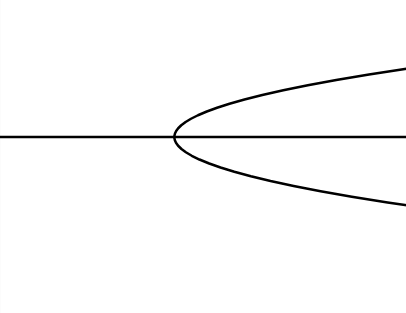
\includegraphics[width=0.48\textwidth]{figures/pitchfork_1.png}\hfill
    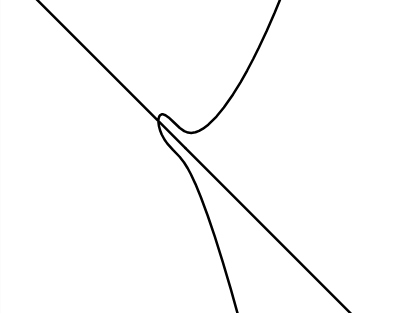
\includegraphics[width=0.48\textwidth]{figures/pitchfork_2.png}
    
    \caption{La pitchfork avant et après la transformation, notez comme cette dernière ne détruit pas l'information "qualitative"}
    \label{fig:pitchfork_globale}
\end{figure}
On peut voir assez rapidement que cette 
relation d'équivalence est pertinente de le 
cadre d'étude de problèmes de bifurcation: 
la matrice $\mathcal{S}$ (en réalité, la germe 
de fonction correspondante...) étant 
inversible, ne change pas l'ensemble 
d'annulation, de plus, si on a un certain 
nombre de solutions en $\lambda_0$, par 
exemple 
$(x_1,\lambda_0)$,...,$(x_n,\lambda_0)$ alors 
cet ensemble va être transporté, via $\phi$ sur 
$(H(x_1,\lambda_0),h(\lambda_0)),\cdots,\\
(H(x_1,\lambda_0),h(\lambda_0))$ et donc,grâce à la structure de $\phi$, elles se trouvent 
sur la même "tranche" $\R^n\times \{h
(\lambda_0)\}$. Si on a une germe 
$g(x,\lambda)$ un peut se demander quelles sont les perturbations qui conservent sa structure, ou plus précisemment, qui ne la font pas changer de classe d'équivalence  pour la relation \ref{GolubEQ}. Soit $p(x,\lambda)$ une germe, considérons la famille $h_t=(g+tp)_{t\in [0,1]}$ 
pour que $p$ soit une perturbation qui conserve la structure, on veut deux choses: d'une part que
\begin{equation*}
    \forall t\in [0,1], h_t\text{ est équivalent à } g 
\end{equation*}  
et d'autre part, on veut que \textit{l'équivalence soit lisse}. Souvenez vous,la relation d'équivalence  \ref{GolubEQ} exige l'existence de  germes difféomorphismes, ainsi, pour tous $t\in [0,1]$, on aura des germes de difféomorphismes $\phi_t$  et $S_t$, on va naturellement exiger que 
\begin{equation*}
    (x,\lambda,t)\mapsto \phi(x,\lambda,t)\text{ et } (x,\lambda,t)\mapsto S(x,\lambda,t)
\end{equation*} 
définissent des germes \textit{lisses}
\begin{remarque}
    Le lecteur attentif pourrait se demander comment il est possible de travailler avec un intervalle fixé \textit{à priori } alors qu'on travaille avec des \text{germes}. Cette imprécision sera levée par lemme de Mather [LEMME]
\end{remarque}

\subsection{détermination finie: généralités}\label{detfin}
C'est le coeur du sujet: on veut 
pouvoir se ramener à l'étude d'un nombre fini de termes du développement de Taylor, comment être sûr qu'on a pas perdu d'information essentielle en tronquant la série ?
Nous introduisons la notion suivante
\begin{definition}
    Si $\mathcal{R}$ est une relation 
    d'équivalence sur $\mathcal{E}(0,\R^n,\R^m)$, on dit que $f$ est $k$-$\mathcal{R}$-\coldef{déterminée} si 
    \begin{equation*}
        \forall g\in \mathcal{E}(0,\R^n,\R^m): j^k g=j^k f, (f,g)\in\mathcal{R}
    \end{equation*}
\end{definition}
Les relations d'équivalences qui nous intéressent seront définies par l'action d'un certain groupe $G$
 \begin{equation*}
    \sim_G : e \sim_Gf \Leftrightarrow \exists g\in G : g\cdot e=f
 \end{equation*}
 Si $G$ agit à droite et $H$ agit à gauche, on définit naturellement l'action de $G\times H$ sur $E$
 \begin{equation*}
    (g,h)\cdot x = g\cdot x \cdot h^{-1}
 \end{equation*}
Le groupe le plus naturel est $d(n)$ l'ensemble des germes de difféomorphismes de $\mathcal{E}(0,\R^n)$, son action sur $\mathcal{E}(0,\R^n,\R^m)$  par composition à droite (resp. à gauche) induit \coldef{l'équivalence droite} (resp. gauche). L'action de $\mathcal{A}=d(n)\times d(m)$ sur $\mathcal{E}(0,\R^n,\R^m)$ induit l'équivalence gauche droite.\\
 On définit le groupe de contact $\mathcal{K}$ comme étant l'ensemble des germes de difféomorphisme des $H\in\mathcal{D}_{n+m}$ telles qu'il existe une $h\in\mathcal{D}_n$ respectant le  diagramme suivant:
\[\begin{tikzcd}
	{(0,\R^{n+m})} & {(0,\R^{n+m})} & \\
	{(0,\R^n)} & {(0,\R^n)} & {\text{avec }\iota(x)=(x,0)}
	\arrow["H", from=1-1, to=1-2]
	\arrow["\pi", from=1-1, to=2-1]
	\arrow["\pi", from=1-2, to=2-2]
	\arrow["\iota", shift left=3, from=2-1, to=1-1]
	\arrow["h", from=2-1, to=2-2]
	\arrow["\iota", shift left=3, from=2-2, to=1-2]
\end{tikzcd}\]
remarquez cela impose que $H$ est de la forme $H(x,y)=(h(x),H_1(x,y))$ en effet 
$H(x,y)=(H_0(x,y),H_1(x,y))$ avec $H_0\in\mathcal{E}^n_{n+m}$, et donc 
\begin{equation*}\label{Structpi}
    \pi\circ H(x,y)= H_0(x,y)=h\circ\pi(x,y)=h(x)
\end{equation*} et que, du fait que 
\begin{equation*}
    H\circ \iota(x)=H(x,0)=(h(x),H_1(x,0))=\iota(h(x))=(h(x),0)
\end{equation*}

On doit avoir que 
\begin{equation}\label{Projo}
    H_1(x,0)=0
\end{equation}
On définit $H\cdot f$ comme étant l'unique germe respectant la condition suivante 
\begin{equation}\label{GraphK}
    (h(x),H\cdot f(h(x)))=H(x,f(x))=(h(x),H_1(x,f(x)))
\end{equation}
Et donc 
\begin{equation}\label{Kequ}
    (H\cdot f)(x)=(H\cdot f)(h (h^{-1}(x)))=H_1(h^{-1}(x),f(h^{-1}(x))) 
\end{equation}


L'équation \ref{GraphK} sert simplement à mettre en évidence le fait que $H$ agit sur $f$ via son \textit{graphe}. Il est fort possible que vous trouviez dans la littérature une définition différente  de $\mathcal{K}$, montrons qu'elles sont équivalentes
\begin{proposition}\label{MATRIXform}
    $f,g$ sont $\mathcal{K}
    $-équivalentes si et 
    seulement s'il existe 
    $S\in\mathcal{E}(0,\R^n,
    \operatorname{GL_{p}(\R)}) 
    $  et $\phi\in\mathcal{D}_
    {n}$ une  tels que 
    \begin{equation*}
        f\circ \phi= S\cdot g
    \end{equation*}
\end{proposition} 
\begin{preuve}
    Bien sûr, s'il existe $\phi$ et $S$ 
    verifiant la condition de l'énoncé, 
    alors $f,g$ sont $\mathcal{K}
    $-équivalentes. 
    Maintenant supposons qu'elles sont 
    $\mathcal{K}$-équivalentes,via \ref{Kequ}, il existe 
    $H\in\mathcal{D}_{n+p}$ tel que 
    \begin{equation}\label{Proprecr}
        g(h(x))=H_1(x,f(x))
    \end{equation}
    via \ref{Projo}, on sait que 
    $H_1(x,0)=(H_{1,1}(x,0),\cdots,H_{1,n
    +m}(x,0))^T=0$. On applique alors 
    \ref{Hadamard} aux $(H_{1,i})_{1\leq i \leq n+m}$
    \begin{equation*}
        H_{1,i}(x,0)=0\Rightarrow \exists \lambda_{i,1}\cdots \lambda_{i,n}\in\mathcal{E}_{n+m} :H_{1,i}=\sum_{j=1}^m \lambda_{i,j}\pi_j 
    \end{equation*}
    Ainsi, $H_1(x,y)=M(x,y)\cdot y$ avec $M$ une matrice de germe lisses. Le fait que $M$ est inversible découle du fait que $H$ est un difféomorphisme et que sa matrice jacobienne est donnée par 
    \begin{equation*}
        \begin{pmatrix}
        \frac{\partial h}{\partial x} & 0 \\
        \frac{\partial H_1}{\partial x} & \frac{\partial H_1}{\partial y}  \\
        \end{pmatrix} 
    \end{equation*}
    On réécrit \ref{Proprecr} 
    \begin{equation*}
        g(h(x))=M(x,f(x))\cdot f(x)\Leftrightarrow g(x)=M(h^{-1}(x),f(h^{-1}(x)))\cdot f(h^{-1}(x))
    \end{equation*}
    Ce qui permet de conclure
\end{preuve}


 On peut alors reformuler le problème de la façon suivante: $f\in\mathcal{E}(0,\R^n,\R^m)$  est $k$-$E$-déterminée si $\operatorname{orb}_G(f)$ contient les germes ayant le même jet d'ordre $k$ que $f$. On veut un équivalent de ce magnifique résultat de théorie des groupes de Lie 
\begin{theobox}{}{}
    Si $G$ est un groupe de Lie, $M$ une variété lisse, si $G$ agit sur $M$ (par exemple) par la gauche et si $V$ est une sous variété connexe et lisse de $M$ alors 
    \begin{equation*}
        \exists m\in M : V \subseteq G\cdot m \Leftrightarrow \forall v\in V, T_v (G\cdot v) \supseteq T_v (V)\text{ et } \dim T_v (G\cdot v) \text{ est toujours la même }
    \end{equation*}
\end{theobox}
la première condition est assez intuitive: en effet si on prend l'exemple d'une surface $S$ présentant une symétrie de révolution selon un axe, $S^1$ agit sur $S$ (via la rotation autour de l'axe central) et les orbites sont alors des cercles. Ainsi une courbe qui vit dans $S$ sera contenue dans une orbite si c'est un cercle qui entoure l'axe de révolution et on remarque que cela revient à exiger qu'en chaque point, l'espace tangent (ici la droite tangente à la courbe) soit inclus dans celui du cercle entourant l'axe de révolution généré par $S^1$ et ce point. En général, on veut que les points  de $V$ "très proches" de $v$ puissent être atteint par des "petites" $G$-transformations, i.e, si on a pas l'inclusion des espaces tangents, on peut "sortir" de l'orbite. La deuxième condition permet d'éviter les situations "dégénérées" où 
\begin{equation*}
    \Bigl\{G\cdot v | v\in V\Bigr\}  
\end{equation*}
n'est pas une variété. On veut donc une notion "d'espace tangent" pour les orbites induites par les actions décrites ci-dessus.\\


dans \cite{damon1984unfolding}, James damon a obtenu a obtenu des résultats de détermination finie pour une large classe d'équivalences sur les germes les "sous-groupes géométriques de $\mathcal{A}$ et $\mathcal{K}$ . Nous allons passer les prochains paragraphes à en exposer les idées

\subsection{déploiements et espaces tangents}

La notion de déploiement remonte à 
René Thom [SOURCE]. Notez que dans la 
suite, nous supposerons $f\in\mathcal{E}^m_n\cdot \mathcal{M}_n$: ça simplifiera les calculs et ce n'est pas une vraie restriction.
\begin{definition} 
    $G\in\mathcal{E}^{m+d}_{n+d}\cdot \mathcal{M}_{n+d}$ est  \coldef{un déploiement à $d$ paramètres} de $f$
    si elle respecte le diagramme suivant:
    \[\begin{tikzcd}
	{(0,\R^n)} & {(0,\R^m)} \\
	{(0,\R^{n+d})} & {(0,\R^{m+d})} \\
	{(0,\R^d)}
	\arrow["f", from=1-1, to=1-2]
	\arrow["\iota"', from=1-1, to=2-1]
	\arrow["\iota", from=1-2, to=2-2]
	\arrow["G"', from=2-1, to=2-2]
	\arrow["\pi"', from=2-1, to=3-1]
	\arrow["\pi", from=2-2, to=3-1]
    \end{tikzcd}\]
    des calculs similaires à \ref{Structpi} permettent de voir que cela impose à $G$ d'être de la forme $G(x,u)=(G_1(x,u),u)$ et 
    $G_1(\cdot,0)=f$
    On pose $\mathcal{U}_d(f)$ l'ensemble des déploiements à $d$ paramètres de $f$.
\end{definition}

\begin{remarque}
    dans la littérature, la notion de déploiement et parfois interchangée avec la notion de \coldef{déformation}. Une déformation $F$ de $f$ est simplement une germe de $\mathcal{E}^{m}_{n+d}$ telle que $F(\cdot,0)=f$. En quelque sorte, le déploiement "mémorise" le paramètre mais pas la déformation.
\end{remarque}

\begin{definition}
    Soit $V\subseteq \mathcal{E}^m_n\cdot \mathcal{M}_n$  et $v\in V$ une \coldef{famille à $d$-paramètres}  $G$   \coldef{ à travers} $v$ \coldef{dans $V$} est un élément de  $\mathcal{U}_d(v)$ tel qu'il existe un représentant de  $G_1$, $\tilde{G}_1$ et un voisinage de 0 $U$ tel que $[\tilde{G_1}(u,\cdot)]\in V$ si $u\in U$. L'ensemble de tel déploiements sera noté $\mathcal{U}_d(v,V)$
\end{definition}

\begin{exemple}
    Si $V=\mathcal{M}^2_1$ et $v(x)=x^3$, alors 
    \begin{equation*}
        G_1(x,u)=x^3+ux^2
    \end{equation*}
    est une famille à 1 paramètres à travers $v$ dans $V$. Mais par exemple 
    \begin{equation*}
        G_2(x,u)=x^3+ux
    \end{equation*}
    ne l'est pas.
\end{exemple}
On va s'intéresser particulièrement aux famille à 1 seul paramètre, c'est à dire les \coldef{chemin lisses} dans une sous "variété"  $V$ de $\mathcal{E}^n_m$.


Rappelons que si $M$ est $N$ sont des variétés lisses et si $f\in C^{\infty}(M,N)$ alors l'ensemble des champs de vecteurs lisses \coldef{le long} de $f$, $\mathcal{V}(f)$ est donné par l'ensemble des $\xi: M\rightarrow TN$
respectant le diagramme suivant: 

\[\begin{tikzcd}
	TM & TN \\
	M & N
	\arrow["Tf", from=1-1, to=1-2]
	\arrow["\pi"', from=1-1, to=2-1]
	\arrow["\pi", from=1-2, to=2-2]
	\arrow["\xi", from=2-1, to=1-2]
	\arrow["f", from=2-1, to=2-2]
\end{tikzcd}\]
On remarque alors que
\begin{equation*}
    \mathcal{V}(f)=\Gamma f^{*} TN
\end{equation*}
Considérons alors le faisceau (c.f remarque \ref{remsheaf} )
des sections locales lisses 
$\Gamma(\cdot,TM)$, l'ensemble des germes de champ de vecteurs en un point $x\in M$ est simplement $\Gamma(\cdot,TM)_x$ et l'ensemble des germes de champ de vecteurs le long de $f$ en $x$ est $\Gamma(\cdot, f^{*}T\R^m)_{x}$

Maintenant, si $f\in\mathcal{E}^m_n$, on entend par $\mathcal{V}(f)$ la germe en $0$ des champs de vecteurs le long d'un représentant de $f$.
du fait que $T \R^m\cong \R^{2m} $, on vérifie facilement que 
\begin{equation*}
    \mathcal{V}(f)=
    \biggr>\frac{\partial }{\partial y_1},\cdots, \frac{\partial  }{\partial y_m}  \biggl<_{\mathcal{E}_n}
\end{equation*}



\begin{definition}
    Soit $V\subseteq \mathcal{E}^m_n$ et $f\in V$ on définit \coldef{l'espace tangent de $v$}
    comme 
    \begin{equation*}
        T_f V =\left\{\frac{\partial G}{\partial u}(0) \biggr| G\in\mathcal{U}_1(f,V) \right\}
    \end{equation*}
\end{definition}

On vérifie aussi facilement que les éléments de $T_f V$ sont bien des vecteurs le long de $f$.

\begin{proposition}
    \begin{equation*}
        T_f \mathcal{K}\cdot f=\cdots
    \end{equation*}
\end{proposition}
\begin{preuve}
    Soit $G\in\mathcal{U}_1(f,\mathcal{K}\cdot f)$, c'est à dire une germe de le forme
    \begin{equation*}
        G(x,u)= (H_u\cdot f(x),u)\text{ avec $H_u\in \mathcal{K}$}
    \end{equation*}
    On peut supposer sans perte de généralité que $H_{0}=\operatorname{Id}$. Via \ref{MATRIXform} et \ref{GraphK}, on écrit 
    \begin{equation*}
        H_u\cdot f(x)=M_u(h_u^{-1}(x),f(h_{u}^{-1}(x)))\cdot f(h_u^{-1}(x))
    \end{equation*}
    Et on calcule alors 
    \begin{equation}
        \frac{\partial G}{\partial u}(0)= 
    \end{equation}

\end{preuve}

\todo{Un théorème de détermination finie}\\
\todo{Le groupe de montaldi}\\
\todo{Classification explicite}\\
\todomaybe{Notion de sous-groupe géométrique}
\newpage

\section{Méthodes topologiques}

\todo{paragraphe introductif}

\subsection{Introduction à la théorie du degré}

Plaçons nous, dans un premier temps, en dimension finie et considérons un ouvert $U$ de $\R^n$, $f\in C^0(\bar{U},\R^n)$ et $y\notin f(\partial U)$ et supposons qu'on veuille construire une fonction $\operatorname{deg}$ qui "compte" le nombre de de solutions de l'équation $f(x)=y$ dans $U$. Faisons une petite analyse de la situation: remarquons d'abord qu'on doit avoir la \coldef{normalité}
\begin{equation*}
    \forall y\in U,\operatorname{deg}(\operatorname{Id},U,y)=1
\end{equation*}

En effet, dans ce cas la seule solution est $x=y$. Mainenant, si on a deux sous ensembles ouverts de $U$, $V_1$ et $V_2$ et qu'ils sont disjoints. Supposons de plus que toutes les solutions soient dans $V_1$ ou $V_2$ et qu'elles sont en nombre fini, alors on aimerait bien avoir \coldef{l'additivité}

\begin{equation*}
    \operatorname{deg}(f,U,y)=\operatorname{deg}(f,V_1,y)+\operatorname{deg}(f,V_2,y)
\end{equation*}

Le lecteur familier avec la topologie trouvera particulièrement naturel d'exiger une notion \coldef{d'invariance par homotopie}. Précisons: on dira que $f$ et $g\in C^0(\bar{U},\R^n)$ sont homotopes si on peut trouver

\begin{equation*}
    H\in C^0([0,1]\times\bar{U},\R^n): H(0,\cdot)=f \text{ et } H(1,\cdot)=g
\end{equation*}
Informellement, on déforme continûment $f$ vers $g$. Attention, on ne peut pas déformer comme on veut, il faut que cette déformation n'affecte pas l'ensemble des solutions. On formule alors une troisième condition, ainsi, si on a 
\begin{equation*}
    H\in C^0([0,1]\times \bar{U},\R^n), y\in C^0([0,1],\R^n): \forall t\in [0,1], y(t)\notin H(t,\partial U)
\end{equation*}
alors  on voudrait que 

\begin{equation*}
    \operatorname{deg}(H(t,\cdot),U,y(t))
\end{equation*}
Soit toujours le même. Notez qu'en plus la fonction, on s'autorise aussi à bouger la "cible", mais on s'interdit de toucher la frontière !
de façon remarquable, en dimension finie, il n'y a qu'une seule fonction qui possède ces propriétés ! On peut donc parler "du" degré. On l'appelle le \coldef{degré de Brouwer}

\begin{definition}
    Si $U\subseteq \R^n$ est ouvert et borné, si $f\in C^0(\bar{U})\cap C^1(U)$ et $y\in \R^n\setminus f(\partial U \cup S_f(U))$ alors on pose 
    \begin{equation*}
        \operatorname{deg}(f,U,y)=\sum_{x\in f^{-1}(y)} \operatorname*{sign} \det df(x)
    \end{equation*}
\end{definition}
On peut montrer que cette fonction remplit bien les 3 
conditions et que c'est la seule. Ensuite, via le 
\colprop{théorème de Morse-Sard} et quelques techniques 
d'approximation classiques, on peut généraliser cette 
fonction à $C^0(\bar{U})$, voir \cite{KlausNonLin85} pour 
les détails. Notez que les 3 conditions mènent à une 
fonction qui ne compte pas vraiment le nombre de 
solutions, mais associe un \textit{signe} à chacune d'entre elles. 


\subsection{Approche historique: le degré de Leray-Schauder}
Il est impossible de généraliser la notion du degré de Brouwer aux espaces de Banach. Pour le voir, nous montrons un cas particulier du théorème du point fixe en utilisant uniquement les propriétés du degré et montrons ensuite qu'il ne s'applique pas en dimension infinie
\begin{proposition}
    si $r>0$ et $f\in C^0(\bar{B(0,r)},\bar{B(0,r)})$ alors $f$ admet un point fixe
\end{proposition}
\begin{preuve}
    S'il existe $x\in\partial \bar{B(0,r)}$ tel que $f(x)=x$, on a terminé. Sinon,
    Considérons 
    \begin{equation*}
        H: [0,1]\times \bar{B(0,r)}\rightarrow \R^n: (t,x)
        \mapsto x-tf(x)\text{ et } y(t)=0
    \end{equation*}
    C'est une homotopie entre $\operatorname{Id}-f$ et 
    l'identité et $0\notin H([0,1]\times\partial \bar{B(0,r)})
    $ car, si $x\in\partial \bar{B(0,r)}$, $H(t,x)=x-f(x)\neq 
    0$ par hypothèse et si $0\leq t<1$
    \begin{equation*}
        |H(t,x)|\geq |x|-t|f(x)|\geq (1-t)r>0
    \end{equation*}
    et donc
    \begin{equation*}
        \operatorname*{deg}(\operatorname{Id}-f,B(0,r),0)
        =\operatorname*{deg}(\operatorname{Id},B(0,r),0)=1
    \end{equation*}
    et donc il existe $x\in B(0,r)$ tel que $x-f(x)=0$
\end{preuve}

Un petit contre exemple en dimension infinie
\begin{exemple}
    Considérons $X=l_\infty$ 
    \begin{equation*}
        f: B(0,1)_{\infty}\rightarrow B(0,1)_{\infty}
    , (x_i)_{i\in\mathbb{N}}\mapsto 
        (1-||x||_{\infty},\sqrt{|x_1|},\sqrt{|x_2|},\cdots)
    \end{equation*}
    On vérifie facilement que $f$ est continue. Supposons donc qu'elle a un point fixe $y$, on aurait alors 
    \begin{equation*}
        y_1= 1- ||y||_{\infty}\text{ et, si $k\geq 2$  } y_k = |y_1|^{\frac{1}{2^{k-1}}}
    \end{equation*}
    Si $||y||_\infty=1$,  alors tous les $y_k$ sont nuls, absurdité. Si $||y||_\infty<1$, alors $y_1$ et la suite converge vers 1, absurdité car cela impliquerait $||y||_{\infty}=1$
\end{exemple}
\begin{corollaire}
    Il n'existe pas d'équivalent au degré de Brouwer en dimension infinie.
\end{corollaire}
Il faut alors restreindre l'ensemble des fonctions sur lequel on va travailler si on veut espérer définir une notion de degré. C'est le travail effectué par  Juliusz Schauder et  Jean Leray pendant les années 30, nous consacrons les prochaines paragraphes à en faire la synthèse.
Le degré de Leray-Schauder est défini sur les \coldef{ perturbations compactes de l'identité} i.e on suppose $F$ de la forme $I-G$ avec $G$ une application compacte , il a alors obtenu le résultat suivant
(qu'on énonce sans preuve) 

\begin{theobox}{Leray-Schauder}{}
    Soit $X$ un espace de Banach et 
    \begin{equation*}
        A=\left\{
            (I-G,U,y): U \subseteq\mathcal{B}(X)\text{ et ouvert },G\in\mathbb{K}(\bar{U}),y\notin (I-G)(\partial U)
        \right \}
    \end{equation*}
    l'ensemble des \coldef{triplets admissibles}
    il existe une unique fonction 
    \begin{equation*}
        \operatorname{deg}: A\rightarrow \mathbb{Z}
    \end{equation*}
    satisfaisant la normalité, l'invariance par homotopie et l'additivité.
\end{theobox}


Avec ce degré, on peut obtenir des résultats globaux de Bifurcation sa construction nécéssite pas mal de lemmes techniques, les démonstrations sont laborieuse et les résultats sont plus faibles que ceux obtenus avec la notion de degré plus récente présentée ci-dessous

\subsection{Le degré de Furi}
\subsubsection{Orientation de fonction de Fredholm d'indice nul}
Nous allons introduire une notion d'orientation pour les fonctions de Fredholm. Cette dernière, proposée par Furi dans \cite{BenevieriFuri1998}, a ensuite été mobilisée dans \cite{BenevieriFuri2001} pour obtenir des résultats de bifurcation. Nous présentons ainsi les idées de ces 2 papiers.
\begin{definition}
    Si $X,Y$ sont des espaces de Banach et  $D\in\mathcal{F}_0(X,Y)$ alors $E\in L(X,Y)$ est un \coldef{correcteur } de $D$ si $D+E$ est un isomorphisme d'espace vectoriel et si son image est de dimension finie. On pose $\mathcal{C}(D)$ l'ensemble des correcteurs de $D$
\end{definition}
On remarque que $\mathcal{C}(D)$ n'est jamais vide, en effet, si on écrit $X=\ker D\oplus X_0$ et $Y=\operatorname*{im} D \oplus Y_0$, on sait que $\ker D$ et $Y_0$ sont isomorphes, notons $A_0$ l'isomorphisme, on remarque alors que 
\begin{equation}\label{correcteur-exemple}
    A:  X\rightarrow Y, x_1+x_2\mapsto A_0(x_1)
\end{equation}
répond à la question. En effet, il est injectif car $Y_0\oplus \operatorname*{im} D=Y$ et il est surjectif car une perturbation de rang fini d'un opérateur de Fredholm ne change pas l'indice.
Dans la suite de cette section on suppose $D$ comme dans la définition précédente.
Avant de pouvoir définir l'orientation, il nous faut une notion de "avoir la même orientation", on fait ça en définissant une relation d'équivalence sur $\mathcal{C}(D)$

\begin{lemme}
    Soient $D\in\mathcal{F}_0(X,Y)$ et $E,E'\in \mathcal{C}(D)$. Si on pose $\phi_{E,E'}=(D+E')^{-1}(D+E)$
    l'opérateur
    \begin{equation*}
        F= \operatorname{Id}_X -\phi_{E,E'}
    \end{equation*}
    a une image de dimension finie
\end{lemme}

\begin{preuve}
   Notons d'abord que 
   \begin{equation*}
        (D+E')F= (D+E')-(D+E)=E'-E
   \end{equation*}
   donc $\im F=\im (E-E')$. Et du fait que 
   \begin{equation*}
        \dim \im (E-E')\leq \dim (E+E')\leq \dim(E)+\dim(E'),
   \end{equation*}
   on conclut.
\end{preuve}




\begin{lemme}
    Soit $F$ comme dans le lemme précédent, alors pour tous $X_0,X_1\subseteq  X$ sous-vectoriels de dimension 
    finie contenant $\im F$
    \begin{equation*}
        \det \phi_{E,E'}|_{X_0}= \det \phi_{E,E'}|_{X_1}
    \end{equation*}
    avec la convention que si $X_0=\{0\}$,  $\det \phi_{E,E'}|_{X_0}=1$
\end{lemme}
\begin{preuve}
    Notez que $\phi_{E,E'} =I-F$ est un isomorphisme, que $(I-F)(X_0)\subseteq X_0$, donc $(I-F)|_{X_0}: X_0\rightarrow X_0$ est un automorphisme d'un espace vectoriel de dimension finie, la notion de déterminant à donc un sens. Supposons d'abord avoir $X_0\subseteq X_1$, on le complémente par $X'_0$, i.e 
    \begin{equation*}
        X_1=X_0\oplus X'_0
    \end{equation*}
    On décompose alors $(I-F)_{X_1}$ comme ceci
    \begin{equation*}
            \begin{pmatrix}
        \operatorname{Id}_{X'_0} & 0 \\
        -\pi_F & (I-F)_{E_0} 
        \end{pmatrix}
    \end{equation*}
où  $\pi_F$ est la projection sur $X_0$ de  $F_{X'_0}$, on conclut immédiatement. Maintenant, dans le cas général, notez que $X_0\cap X_1$ contient $\im F$ et est de dimension finie. On applique alors le résultat obtenu deux fois 
\begin{equation*}
    \det (I-F)|_{X_0}= \det (I-F)|_{X_1\cap X_0}=\det (I-F)|_{X_1}
\end{equation*}
\end{preuve}



\begin{definition}
    dans les conditions des deux lemmes précédents, on dit que les correcteurs  $E$ et  $E'$  sont $D$-\coldef{équivalents} si $\det (\phi_{E,E'})|_{X_0}>0$, on écrira  $E\sim_{D} E'$
\end{definition}
\begin{proposition}
    $\sim_D$ est une relation d'équivalence sur $\mathcal{C}(D)$
\end{proposition}
\begin{preuve}
    La réfléxivité et la transitivité sont évidentes,on montre alors la transitivité. Soient donc $E,F,G\in\mathcal{C}(D)$ tels que $E\sim_D F$ et $F\sim_D G$ on considère alors un sous vectoriel de dimension fini $X_0$ content les images de $I-\phi_{E,F},I-\phi_{F,G},I-\phi_{E,G}$ , il suifft alors de remarquer que 
    \begin{equation*}
        \det \phi_{E,G}|_{X_0}=
        \det \phi_{F,G}\phi_{E,F}|_
        {X_0}=
        \det \phi_{F,G}|_{X_0}
        \cdot \det \phi_{E,F}|_
        {X_0}>0
    \end{equation*}
    donc $E\sim_{D} G$ 
\end{preuve}

Il  de plus clair que cette relation d'équivalence partitionne 
$\mathcal{C}(D)$ en deux classes d'équivalence. Notez que si $D_1$ et $D_2$ peuvent être composés et que si $E_1$ et $E_2$ sont des correcteurs de $D_1$ et $D_2$ respectivement, alors $D_2E_1+ E_2E_1+ E_2D_1$ est un correcteur de $D_2D_1$, de fait 

\begin{equation*}
    D_2D_1+ D_2E_1+ E_2E_1+ E_2D_1 =(D_1+E_1)(D_2 + E_2)
\end{equation*}


\begin{definition}
    Une \coldef{orientation} de $D\in\mathcal{F}_0(X,Y)$ est une des 2 classes d'équivalence de $\mathcal{C}(D)$. Un \coldef{opérateur orienté} est une paire $(D,c)$ où $c$ est une oreitnation. Si $(D,c)$ est orienté, un correcteur sera dit \coldef{positif} s'il est dans $c$ et négatif sinon. On pose alors $\mathcal{C}_{+}(D)$ l'ensemble des correcteurs positifs et $\mathcal{C}_{-}(D)$ les négatifs. Lorsque $D$ est un isomorphisme, $0$ est un correcteur, on définit alors \coldef{l'orientation naturelle} $\nu(D)$ de $D$ comme étant la classe d'équivalence contenant $0$. Si $(D,c)$ est isomorphisme orienté, on pose $\operatorname{Sign}D=1$ si $0\in c $, et $-1$ sinon 
\end{definition}
\begin{definition}
    Si $(D_1,c_1)$ et $(D_2,c_2)$ sont des opérateurs orientés, on note $c_2\circ c_1$ l'orientation de $D_2\circ D_1$ telle que
    \begin{equation*}
        D_2E_1+ E_2E_1+ E_2D_1\in  c_2\circ c_1
    \end{equation*}
    où $E_1\in c_1$ et $E_2\in c_2$. On vérifie 
    facilement que ça ne dépend pas du choix des 
    $E_1$, $E_2$ La composition de deux opérateurs 
    orientés sera, sauf si mention du contraire, 
    la précédente. 
\end{definition}

Il est enrichissant de remarquer 
que la catégorie $\mathcal{G}(D)$ 
ayant pour objets les éléments de 
$\mathcal{C}(D)$ et comme 
morphismes les $(\phi_{E,F})_{E,F\in\mathcal{C}(D)}$ est un groupoïde. Si on considère la catégorie correspondant à $\mathbb{Z}_2$, i.e la catégorie n'ayant qu'un seul objet $o$ , $+1,-1$ comme morphismes et la multiplication comme loi de composition , qu'on note $\mathbf{B}\mathbb{Z}_2$
\footnote{C'est le "delooping" du groupe $\mathbb{Z}_2$, le lecteur intéressé peut consulter l'article nLab \url{ https://ncatlab.org/nlab/show/delooping} }
alors 

\begin{equation*}
    \operatorname*{Sign}: \mathcal{G}(D)\rightarrow \mathbf{B}\mathbb{Z}_2, E\mapsto o, \phi_{E,E'}\mapsto \operatorname*{sgn}\det \phi_{E,E'}|_{X_0}
\end{equation*}

est un foncteur donc $\mathcal{G}^+(D)$, la catégorie $\mathcal{G}(D)$ ou on retire les les morphismes dont le determinant restreint est négatif, est un sous groupoïde (c'est même un sous groupoïde normal) de $\mathcal{G}(D)$. Il est clair que ce groupoïde à axactement deux composantes connexes, qui correspondent donc aux choix possibles d'orientation\\
Soit $(D,c)$ un opérateur orienté, via Hanh-Banach, on peut supposer que le correcteur $A$ donné en \ref{correcteur-exemple} est continu, on peut de plus supposer qu'il est positif. Maintenant, $D+A$ est un isomorphisme d'espaces de Banach et il existe un voisinage (pour la topologie des opérateurs) $V_D$ tel que si $D'\in V_D$, alors $A$ est un correcteur de $D'$, on appelle alors \textcolor{color-def}{l'orientation induite par $(D,c)$} sur $D'$ celle qui fait de $A$ un correcteur positif \\
On définit maintenant l'orientation pour une famille continue d'opérateurs de Fredholm
\begin{definition}
    Soit $(\Lambda,\mathcal{T})$ un espace topologique et $h\in C^0(\Lambda,\mathcal{F}_0(X,Y))$,
    $\alpha_{\lambda}$
    est une 
     \textcolor{color-def}{orientation} 
    si  pour tout $\lambda\in\Lambda$, $\alpha_{\lambda}\in\mathcal{C}(h(\lambda))/\sim_{h(\lambda)}$ et il existe $A_{\lambda}\in\alpha_\lambda$ qui est correcteur positif (pour l'orientation induite) de $h(\lambda')$ si $\lambda'$ est dans un voisinnage de $\lambda$. Une famille est alors dite \textcolor{color-def}{orientable} si il existe une orientation. Un sous ensemble $\mathcal{D}$ d'opérateurs de Fredholm d'indice 0 est orientable si l'inclusion $\iota : \mathcal{D}\rightarrow \mathcal{F}_0(X,Y)$ est orientable
\end{definition}

\begin{lemme}
    Dans les condition de la définition précédente, si $\Lambda$ est connexe, et si $h$ est orientable, alors $h$ admet exactement deux orietations 
\end{lemme}

\begin{preuve}
    Soit $\alpha_\lambda$ une orientation de $h$, et supposons que $\alpha'_\lambda$ coïncident avec $\alpha$ sur une partie $\Omega$ de $\Lambda$ et montrons qu' $\Omega$ est ouvert. Soit alors $\lambda_0\in\Omega$, par définition, il existe des voisinages de $\lambda_0$ $V_1$,$V_2$ et $A_1\in\alpha'(\lambda_0)$, 
    $A_2\in\alpha'(\lambda_1)$ qui sont des correcteurs positifs pour $h(\lambda')$ si $\lambda'$ est dans $V_1$ ou $V_2$, respectivement. Il suffit alors de remarquer que $\alpha$ et $\alpha'$ coïncident sur $V_1\cap V_2$. De façon identique, l'ensemble sur lesquels les orientations sont opposées est un ouvert, on conclut immédiatement
\end{preuve}

\begin{remarque}
    Notez que cette notion d'orientabilité est une généralisation de la notion d'orientabilité d'une variété plongée $M$ de dimension finie $n$: en effet, il suffit de considérer
    \begin{equation*}
        h: M\rightarrow L(\R^n,\R^n), x\mapsto \pi^{N_x} 
    \end{equation*}
    avec  $\pi^{N_x}$ la projection sur l'espace normal $N_xM$
\end{remarque}

\begin{definition}
    Soit $U\subseteq X$ un ouvert et $F: U\rightarrow X$ une fonction de Fredholm d'indice zéro. Une \textcolor{color-def}{orientation} de $F$ est simplement une orientation de $DF$ , et $F$ est \textcolor{color-def}{orientable} si $DF$ l'est. Si $F$ est un difféomorphisme, alors $F$ possède une orientation naturelle, notée $\nu$
\end{definition}

\subsubsection{Construction du degré de Furi}

On peut maintenant construire le degré de Furi 
\begin{definition}
    Soit $F:X\rightarrow Y$ une fonction orientable et $y\in Y$, le triplet $(F,X,y)$ est 
    \textcolor{color-def}{admissible} si $F^{-1}(y)$ est compact. Si $U$ est un ouvert de $X$, on dit que le triplet $(F,U,y)$ est
    \textcolor{color-def}{admissible} si $F^{-1}(y)\cap U$ est compact et \textcolor{color-def}{fortement admissible } si $F$ admet une extension $F'$ continue $\bar{U}$, propre, et telle que $y\notin F(\partial U)$
\end{definition}

Du fait que les fonctions de Fredholm sont localement propre \ref{propre-fred}, l'admissiblité du triplet $(F,X,y)$ implique l'existance d'un voisinnage ouvert de $F^{-1}$ qui rend le triplet $(F,U,y)$ fortement admissible 

\begin{definition}
    Soit $U\subseteq X$ un ouvert et  $H\in C^0(U\times [0,1])$ continûment dérivable par rapport à la première variable. $(H,\alpha)$ est une \coldef{homotopie orientée} si $\alpha$ est une orientation de $D_1 H$
\end{definition}

On adapte alors les propriétés qu'on voudrait avoir pour  le degré \\
Les conditions d'\coldef{additivité} et de \coldef
{normalité} restent les mêmes que pour le degré de Brouver \coldef{L'invariance par 
homotopie} devient une \coldef{invariance par homotopie 
orientée}:\\  Soit $H: X\times [0,1]\rightarrow Y$ une homotopie orientée et $y\in C^0([0,1],Y)$, si l'ensemble 
\begin{equation*}
    \left\{(x,t)\in X\times [0,1]: H(x,t)=y(t) \right\}
\end{equation*}
est compact alors $\deg (H_t,X,y(t))$ est bien défini pour et ne dépend pas de $t\in [0,1]$\\
La propriété suivante est évidente pour le degré de Brouwer, mais à expliciter  en dimension infinie, il s'agit de \coldef{l'invariance topologique}: Si $(F,X,y)$ est admissible et $\varphi: W\rightarrow X$, $\psi: Y\rightarrow Z$ sont des difféomorphismes naturellement orientés alors 
\begin{equation*}
    \deg(F,X,y)=\deg(\psi F \varphi, W, \psi(y))
\end{equation*}

Enfin, une propriété qui nous permet de faire l'analogue de l'analogue de la réduction de Lyapunov-Schmidt, nous la donnons à titre indicatif
\begin{definition}
   Sit $Y_0$ est un sous espace de $Y$,  $F:X\rightarrow Y$ est \coldef{transverse} à $Y_0$ si 
   \begin{equation*}
    \forall x\in F^{-1}(Y_0), Y_0+\im DF(x)=N.
   \end{equation*}
\end{definition}
\coldef{Réduction}: si $F:X\rightarrow Y$ est orientée, et si $Y_0$ est transverse, alors on pose  $f_1$ la restriction de $f$ à $X_0=f^{-1}(Y_0)$, alors on veut que
\begin{equation*}
    \deg (f,X,y)=\deg(f_1,X_0,y)
\end{equation*}
\begin{theobox}{}{}
    Soit $U$ un ouvert de $X\times\Lambda$, $F:U\rightarrow Y$ une famille d'index zéro et ayant une branche triviale de solutions et soit $A\in\mathcal{C}(DF(x_0,\lambda_0)) $ si la fonction 
    \begin{equation*}
        f: \R\rightarrow\R, \lambda\mapsto \det ((dF(0,\lambda)+A)^{-1}DF(0,\lambda))
    \end{equation*}
    change de signe en $\lambda_0$, alors c'est un point de bifurcation. 
\end{theobox}
\begin{preuve}
    \todo{PREUVE complete}
\end{preuve}
\subsubsection{Un résultat global via le degré orienté}
\todo{LEMMES}
\begin{theobox}{Furi}{}
    dans les conditions du théorème précédent, si $F$ est 
    orientable alors il existe un ensemble connexe de 
    solutions non-triviales $S$ tel que son adhérence dans 
    $U$ contiennent $(0,\lambda_0)$ et est soit non-compacte, 
    soit contient $(0,\lambda_1)$ avec $\lambda_0\neq 
    \lambda_1$
\end{theobox}
\begin{preuve}
    \todo{PREUVE complete}
\end{preuve}

\newpage
\section{Introduction aux bifurcations dynamiques}
\subsection{Quelques notions de stabilité}
Jusqu'ici, on s'intéressait au changement du lieu d'annulation d'une fonction $F$. Dans un contexte de dynamique, ça correspond à étudier la façon dont les points d'équilibre changent lorsqu'un paramètre varie, et on "oubliait" en quelque sorte la dynamique dont était originaire la fonction, ce qui invisibilise certaines propriétés de ces équilibres. Reprenons la dynamique de l'exemple \ref{Poutre}, en considérant le premier mode de flambement
\begin{equation*}
    F(\theta,\lambda)=D^2 \theta + (\lambda+n^2\pi^2) \sin\theta =0
\end{equation*}

Intuitivement, on sent bien que si on dépasse la valeur 
critique, alors la poutre va \textit{forcément} se tordre 
(dans une des 2 directions !) et qu'il est impossible que 
le système reste sur la ligne triviale. On a donc bien 
envie de pouvoir distinguer les "vrais" équilibres, 
physiquement réalistes, et ces équilibres "fantômes" qui 
n'existent que mathématiquement. C'est là que la notion de 
\textit{stabilité} intervient : les solutions de la branche 
triviale, une fois la valeur critique dépassée, sont 
\textit{instables}. Nous allons maintenant donner un sens précis à la notion de stabilité et comprendre comment l'utiliser pour des problèmes de bifurcation. Nous verrons que pour ce faire, il faudra étudier le spectre de la dérivée de Fréchet.\\
Bien qu'on travaille avec des espaces de Banach  réels, il est très courant de passer par le complexifié pour l'étude du spectre. Cette section est adaptée de \cite{henry1981geometric}. Dans ce qui suit, $D:X\rightarrow X$ est un endomorphisme d'espace de Banach.
\begin{definition}
    Si $V$ est un espace vectoriel, le \coldef{complexifié} $V^{\mathbb{C}}$ de $V$ est donné par 
    \begin{equation*}
        V^{\mathbb{C}}=V\otimes_{\R}\mathbb{C}\cong V\oplus i V=\left\{ v_1+iv_2\big| v_1,v_2\in V\right\}
    \end{equation*}
\end{definition}
Si $X$ est un espace de Banach, on munit habituellement son complexifié de la norme 
\begin{equation*}
    ||x+iy||_{X^\mathbb{C}}= \sup_{\theta\in[0,2\pi]} ||x\cos\theta + y\sin \theta ||
\end{equation*}
On vérifie facilement que cette dernière en fait un espace 
de Banach. Quand on parle du spectre de l'opérateur $D$, on parle en réalité de l'opérateur complexifié 
\begin{equation*}
    D^{\mathbb{C}}: X^{\mathbb{C}}\rightarrow X^{\mathbb{C}}
, x+iy\mapsto Dx +iDy
\end{equation*}
\begin{definition}
    On définit $\sigma(D)$ \coldef{le spectre} de $D$ comme étant l'ensemble des complexes $\lambda$ pour lesquels $D$ n'est pas inversible. On décompose ce dernier en trois composantes : 
    \begin{itemize}
        \item le spectre ponctuel $\sigma_p(D)$
        \item le spectre continu $\sigma_c(D)$
        \item le spectre résiduel $\sigma_r(D)$
    \end{itemize}
    on définit enfin \coldef{résolvant} comme étant le complémentaire  $\rho(D)$ du spectre.
\end{definition}

\begin{definition}
    Soit
    \begin{equation*}
        \Sigma_{\omega,c}=\left\{ \lambda\in\mathbb{C}\big|
        \omega\leq |\arg(\lambda-c)|\leq \pi,\lambda\neq c\right\}
    \end{equation*}
    le secteur de centre $c$ et d'ouverture $\omega$.
    $D$ est $\omega,c$-\coldef{sectoriel} avec $a$ réel et $\omega\in ]0,\frac{\pi}{2}[$ si 
    \begin{equation*}
        \Sigma_{\omega,c}\subseteq \rho(D)\text{ et } 
        \sup_{\lambda\in\Sigma_{\omega,c}}\frac{||(\lambda-D)^{-1}||}{|\lambda-c|} < \infty
    \end{equation*}

\end{definition}

\newpage
\subsection{La bifurcation de Hopf}
\newpage


\newpage

\addtocategory{utilises}{dieudonne1969fma8,BenevieriFuri1998,BenevieriFuri2001,kato1995pto,coleman2012calculus,kielhoefer2012bta,golubitsky1985sgb1,golubitsky1988sgb2,montaldi2021sbc,Feckan2008Topological,Kawanago2023HopfBanach,Marx1994Bifurcation,Karoubi1978KTheory,Wall1981Finitedeterminacy,Marcut2009FredholmNotes,KlausNonLin85,friedmanpartial,damon,abramovich2002invitation,EsserFONCT,henry1981geometric}
\addtocategory{plusloin}{schwartz1960nash,glockner2006implicit}
\printbibliography[
  category=utilises,
  title={Références utilisées}
]

\printbibliography[
  category=plusloin,
  title={Pour aller plus loin}
]

\end{document}